\chapter{Methods}\label{ch_methods}

The preceding chapters established that no existing tool jointly optimises map styles and tile data, and introduced the compiler, database, and encoding techniques whose analogues make such joint optimisation possible.
This chapter applies those foundations to the design and implementation of our concrete optimiser - a standalone Rust tool that consumes a MapLibre style~JSON document and, optionally, tile-level statistics, and produces a visually equivalent style together with optimised tile data.

The chapter proceeds as follows.
\cref{sec_problem_statement} formalises the optimisation problem and the visual-equivalence constraint that all passes must satisfy.
\cref{sec_scope} scopes the work to MapLibre GL~JS and describes the implementation platform.
\cref{sec_approach} then describes the three-level pipeline, and the subsequent sections detail the individual passes at each level.

\section{Formalised Problem Statement}\label{sec_problem_statement}

With the foundations established in \cref{ch_theoretical_background}, the optimisation problem addressed by this thesis can be stated formally.
Let $\mathcal{S}$ be the set of syntactically valid MapLibre style~JSON documents, and $\mathcal{T}$ be the set of tile sets (a tile set is a finite family of tiles indexed by source, $x$, $y$, $z$).
Let $\mathcal{V}$ be the set of \emph{viewing states} a renderer can be in - roughly, $(x, y, z, \text{pitch}, \text{bearing}, \text{viewport size})$ tuples - and let
\begin{equation}\label{eq:render_function}
    R : \mathcal{S} \times \mathcal{T} \times \mathcal{V} \to \mathcal{I}
\end{equation}
denote MapLibre's rendering function, which maps a style, a tile set, and a viewing state to a rasterised image in $\mathcal{I}$.

The optimiser solves the following problem: given an input pair $(S, T)$ and a cost function $c : \mathcal{S} \times \mathcal{T} \to \mathbb{R}_{\geq 0}$, find $(S', T')$ minimising $c(S', T')$ subject to the \emph{visual equivalence} constraint
\begin{equation}\label{eq:visual_equivalence}
    \forall v \in \mathcal{V}:\; R(S, T, v) \equiv R(S', T', v),
\end{equation}
where $\equiv$ denotes pixel-identity under a deterministic rasteriser.

In practice, $v$ is quantified only over the discrete grid of integer zoom levels and axis-aligned viewports, and pixel-identity is verified by direct image comparison rather than by proof.
The cost function $c$ encodes the deployment-relevant metrics discussed in \cref{sec_benchmarking}; this thesis does not attempt to collapse them into a scalar, instead reporting the effect of each pass on each metric separately.

The constraint~(\cref{eq:visual_equivalence}) is the \emph{soundness criterion} for every pass in this chapter:
Any rewrite whose correctness depends on a MapLibre runtime invariant must either preserve the invariant or reject the rewrite when the invariant cannot be established.
For example, the stats-driven folding pass cannot soundly remove a \texttt{match} arm without a full census of the tile data, because the arm may be reached by features the statistics have not observed; the pass is consequently gated on a sample rate of~1.0 (a full census).
Similarly, the metadata-refinement pass must reason about overzoom (\cref{sec_tiles}) when tightening \texttt{maxzoom}, because an overzoomed tile counts as a viewing state in~(\ref{eq:visual_equivalence}).

\section{Scope}\label{sec_scope}

As discussed in \cref{sec_styles}, the most common target for performance research on interactive maps is a system built on a rich, dynamic style specification.
Two implementations dominate this space: Mapbox~styles and MapLibre~styles.
Since the Mapbox codebase is proprietary and evaluations may not be performed without explicit consent, only MapLibre is a viable research target.

Among MapLibre renderers, the web implementation (\texttt{maplibre-gl-js}) offers the most complete support for the styling language and is the most widely used \emph{as an interactive developer target}: the mobile MapLibre Native renderers share much of the styling engine, but the web renderer is the reference implementation that first tracks new specification features, exposes the richest instrumentation hooks for Puppeteer-driven benchmarking, and runs on the same hardware profile as the benchmark host.
It was therefore selected as the system under test for all rendering benchmarks.

The optimiser itself is a standalone Rust binary.
It takes a style~JSON file as input, applies a configurable set of optimisations passes, and writes an optimised style~JSON as output.
When tile statistics are provided (via an MBTiles database or a pre-computed statistics file), additional data-driven passes become available.
No integration with a specific tile server is required; the optimised artefacts can be served by any standards-compliant tile infrastructure.

The tile re-encoder described in \cref{sub_data_optimisations} lives in the same Cargo workspace as the style optimiser, but is deliberately split into three crates so that it can also be consumed from a \ac{JVM}-based tile-generation pipeline without re-implementing the encoder.
The core encoder and decoder live in \texttt{rust/mlt-core}; the cross-language surface is generated by \emph{Diplomat}~\cite{AuroraRFC77Diplomat}, which produces idiomatic, language-specific bindings directly from annotated Rust types, replacing the earlier \texttt{cbindgen}/\texttt{jextract} approach; and \texttt{rust/mlt-java} wraps the generated bindings as a Java library using the Panama \ac{FFM} \ac{API}.
Panama was chosen over conventional \ac{JNI} glue because it removes the need for hand-written C stubs and gives the \ac{JVM} direct, zero-copy access to off-heap buffers - exactly the boundary shape that a columnar encoder needs, because each tile is handed over as a batch of parallel \texttt{MemorySegment}s rather than one call per feature, amortising the per-boundary cost over thousands of features in one encoder invocation.
The legacy self-contained Java encoder in \texttt{java/mlt-core}~\cite{tremmelMapLibreTileNext2025} is kept only as a reference baseline for the \ac{MLT} experiments in \cref{ch_experiments} and is not a target of the optimisations proposed in this thesis.

\section{Approach}\label{sec_approach}

To evaluate the effectiveness of the optimisations strategies developed in this work, a benchmarking-driven approach was adopted.
A reliable performance baseline was established first, followed by cumulative ablation experiments that isolate the contribution of each optimisations pass.
Each pass preserves the visual-equivalence constraint formalised in \cref{sec_problem_statement}; together, the passes from~\cref{sub_pipeline} seek to minimise $c(S', T')$ across the metrics defined in \cref{sec_benchmarking}.

\subsection{Three-Level Optimisation Pipeline}\label{sub_pipeline}

\Cref{fig:system_architecture} sketches the optimiser system as a whole.
At the centre sits the \emph{Optimiser}, a pipeline of passes at three levels of abstraction.
Around it are three supporting components, each detailed in its own section: a code-generation front end (\cref{sub_codegen}) that produces typed Rust types from the upstream MapLibre style specification; a tile-statistics scanner (\cref{sub_tile_statistics}) that profiles \ac{MVT} tiles for the stats-driven and data-level passes and a validation harness - pixel-exact render tests plus a curated style corpus - that exercises both pipelines against the visual-equivalence guarantee of \cref{eq:visual_equivalence}.
The three pass levels at the centre are:

\begin{enumerate}
    \item \textbf{Expression passes} (\cref{sub_expression_optimisations}) operate directly on the JSON representation of style expressions, applying peephole rewrites, constant folding, and algebraic simplifications without deserialising the style into typed structures.
    They run to a fixpoint with a hard cap of eight iterations; in practice every style in the benchmarking and Maputnik corpora converges within two to three iterations, well below the cap, because human-authored styles tend to reuse a small repertoire of patterns.
    The formal termination measure and confluence discussion are given alongside the pass descriptions.
    \item \textbf{Structural passes} (\cref{sub_structural_optimisations}) deserialise the style into the typed Rust spec produced by the codegen front end and apply transformations that require cross-layer or cross-source reasoning -- dead layer elimination, metadata refinement, layer merging, and cleanup.
    A cross-phase \emph{filter-to-property constant propagation} -- substituting equality constraints extracted from a layer's filter into that layer's paint and layout expressions -- bridges the expression and structural phases and is detailed in \cref{sub_structural_optimisations}.
    \item \textbf{Data passes} (\cref{sub_data_optimisations}) transform the served tile data via a style-driven pruning advisory and the conversion from \ac{MVT} to \ac{MLT}.
\end{enumerate}

\noindent The ordering is a deliberate resolution of the \emph{phase ordering problem}~\cite{clickCombiningAnalysesCombining1995}.
Expression passes run first so that structural passes operate on already-simplified expressions, dead elimination precedes layer merging so that gaps left by removed layers expose new merging opportunities, and the data phase consumes the fully optimised style so that the pruning advisory reflects the final set of live layers and properties.

\begin{figure}[htbp]
    \centering
    \begin{tikzpicture}[
        node distance=0.8cm and 1.4cm,
        box/.style={rectangle, draw, rounded corners=2pt, minimum height=0.7cm,
                    minimum width=2.0cm, font=\small, align=center},
        src/.style={box, fill=blue!12},
        mir/.style={box, fill=violet!12},
        gen/.style={box, fill=green!10},
        data/.style={box, fill=orange!10},
        opt/.style={box, fill=yellow!12, minimum width=2.4cm},
        test/.style={box, fill=red!12},
        arrow/.style={-Stealth, thick},
        query/.style={-Stealth, thick, densely dashed},
        label/.style={font=\scriptsize\itshape, text=gray},
        validationlabel/.style={font=\scriptsize\itshape, text=red},
        validation/.style={
            dashed,
            red,
            ->,
            every edge node/.append style={text=red}
        },
    ]
        % Codegen pipeline (top row)
        \node[src]  (v8)     {\texttt{v8.json}};
        \node[mir,  right=of v8]   (parsed) {ParsedSpec};
        \node[mir,  right=of parsed] (mir)    {MIR};
        \node[gen,  right=of mir]  (serial) {SerialSpec\\{\scriptsize (generated Code)}};

        \draw[arrow] (v8)     -- node[above, label] {decode} (parsed);
        \draw[arrow] (parsed) -- node[above, label] {normalise} (mir);
        \draw[arrow] (mir)    -- node[above, label] {generate} (serial);

        % Data pipeline (bottom row)
        \node[src, below=2.5cm of v8] (proto) {Protobuf\\{\scriptsize (\acs{MVT})}};
        \node[data, right=of proto] (mvt) {MVTLayer};
        \node[data, right=of mvt]   (scan) {DataScanner};

        \draw[query] (proto) -- node[above, label] {decode} (mvt);
        \draw[query] (mvt)   -- node[above, label] {scan tiles} (scan);

        % tangled nodes
        \node[opt, below=2.5cm of serial] (opt) {Optimiser};
        \node[test] (test)  at ($(serial)!0.5!(opt) + (3cm,0)$)  {Render tests};
        \node[test, below=1cm of mir] (corpus) {Style Corpus};

        % tanlged arrows
        \draw[<->,double,thick,densely dashed] (opt) -- node[left,black] {\scriptsize\itshape optimise} (serial);
        \draw[query] (scan) -- node[above, label] {statistics} (opt);
        \draw[validation] (corpus) -- node[left, validationlabel] {validate} (serial);
        \draw[validation] (corpus) -- node[left, validationlabel] {eval} (opt);
        \draw[validation] (test) -- node[right, validationlabel] {validate} (serial);
        \draw[validation] (test) -- node[right, validationlabel] {validate} (opt);
    \end{tikzpicture}
    \caption{System architecture.
    The \emph{codegen pipeline} (top) transforms the upstream \texttt{v8.json} style specification through three stages into generated Rust types (\texttt{SerialSpec}) used for typed style manipulation, with the MIR providing spec metadata to the optimiser.
    The \emph{data pipeline} (bottom) decodes \acs{MVT} tiles and scans them to produce tile statistics that feed into data-driven optimisations passes. Render tests validate round-trip correctness and the style corpus is used to both validate the codegen and evaluate the optimiser.}
    \label{fig:system_architecture}
\end{figure}

\subsection{Code Generation from v8.json}\label{sub_codegen}

Structural passes operate on Rust types \emph{generated} from the upstream MapLibre GL~JS style specification rather than raw JSON.
This shifts spec drift from a manual synchronisation burden to a regenerator invocation, and gives every pass typed access to defaults, value types, and expression capabilities.
A hand-written shadow of the specification is not viable because MapLibre publishes the spec in its own JSON-based \ac{DSL}.

The generation pipeline (top row of \cref{fig:system_architecture}) proceeds in three stages: the published \texttt{v8.json} is \emph{decoded} into an internal representation; the result is \emph{normalised} into a stable intermediate representation - the \texttt{MIR} - that resolves cross-cutting concerns (in particular, paint and layout properties that the spec defines across multiple sections are collapsed into per-layer field definitions carrying type, default, and expression-capability metadata); finally, a code emitter \emph{generates} Rust sources with round-trip serialisation support.
The alternative - hand-written Rust types - would require manual synchronisation with specification changes and risk silent divergence.
Due maplibre being specified in its own, json based \ac{DSL}, a simpler version was not possible.

This metadata is the substrate for two structural passes.
Layer merging queries the MIR to decide whether a differing paint property supports feature-driven expressions - and can therefore be wrapped in a \texttt{case}/\texttt{match} over the filter discriminator - or is camera-only and must remain uniform across merged layers.
Default stripping compares property values against the specification defaults encoded in the generated types.

\subsection{Building Optimisations}\label{sec_building_optimisations}

The implemented passes target three areas of the rendering pipeline: style expressions, structural properties, and tile data.
Each pass is classified by \emph{where} it operates and its \emph{data requirements} (none, sampling, or full scan); many are analogues of well-known compiler and query-processing techniques.
The visual-equivalence constraint of \cref{sec_problem_statement} is the soundness criterion for every pass; how each rewrite preserves it is argued in the per-pass paragraphs below.

For soundness, every pass must independently satisfy the visual-equivalence constraint of \cref{sec_problem_statement}: the optimised output $(S', T')$ must produce pixel-identical rendering for every viewing state.
For expression-level passes, this is witnessed by the termination measure $\mu(S)$ (\cref{eq:termination_measure}): each rewrite strictly reduces $\mu$ while preserving expression semantics.
For structural passes, soundness is argued per-pass in the paragraphs below - dead elimination preserves equivalence because it only removes layers that produce no visible output; metadata refinement preserves equivalence because it only tightens bounds that the renderer would enforce anyway (with the overzoom asymmetry detailed below); layer merging preserves equivalence via the three invariants of \cref{sub_structural_optimisations}.
For data-level passes, the pruning advisory removes only data that no live style layer references, so the rendering function $R$ receives the same effective input.

\subsubsection{Expression-Level Optimisations}\label{sub_expression_optimisations}

Expression passes operate directly on the JSON representation, applying rewrites that reduce expression complexity and eliminate redundant computation.
\cref{tab:expression_passes} summarises the implemented passes.

\begin{table}[htbp]
\centering
\begin{tblr}{
  colspec = {p{3.8cm} p{1.8cm} p{9.5cm}},
  rows = {font=\small},
  row{1} = {font=\small\bfseries},
}
\toprule
Pass & Data & Description [compiler analogy] \\
\midrule
Unary simplification         & none     & Unwrap single-argument \texttt{any}/\texttt{all} wrappers [identity elimination] \\
Expression kind normalisation & none     & Rewrite negated comparisons to their direct form, e.g.\ \texttt{["!",["==",a,b]]} $\to$ \texttt{["!=",a,b]} [operator strength reduction] \\
Constant folding              & none     & Evaluate statically determinable expressions: boolean algebra, dead branch elimination, redundant coercion removal [constant folding, \acs{SCCP}] \\
Stats-driven constant folding & sampling & Fold \texttt{has}/\texttt{get}/\texttt{geometry-type} expressions using tile statistics; prune unreachable \texttt{match}/\texttt{in} arms; fold comparisons against known value ranges [sparse conditional constant propagation] \\
Expression simplification     & none     & De~Morgan's laws, boolean flattening, coalesce flattening, \texttt{case}$\to$\texttt{match} rewriting, \texttt{let}/\texttt{var} inlining, \texttt{any}$\to$\texttt{in} merging, interpolate/step collapsing [algebraic simplification] \\
Default stripping             & none     & Remove paint/layout properties whose value equals the specification default [dead store elimination] \\
Colour minification           & none     & Compress colour literals to their shortest representation [literal compression] \\
Selectivity reordering        & sampling & Reorder filter predicates by selectivity so the most discriminating condition is evaluated first [predicate reordering] \\
\bottomrule
\end{tblr}
\caption{Expression-level optimisations passes.}
\label{tab:expression_passes}
\end{table}

Among these passes, constant folding is expected to dominate because reducing an expression to a literal eliminates all per-feature evaluation cost; the other passes primarily shorten the evaluation path rather than eliminating it.

The expression pass engine is organised as a table of rewrite rules (\cref{tab:all_rewrite_rules}), each gated by a \emph{pass flag} (which pass must be enabled) and scoped to a \emph{rule scope} (whether the rule applies to filters only, to paint/layout properties, or to both).
Selectivity reordering is implemented as a separate pass that runs after the rewrite table has stabilised.
Rules are further classified by their \emph{type}: \emph{pure} rules operate on the expression array alone, \emph{MIR-aware} rules additionally consult the specification's type metadata (e.g.\ to determine whether an operator is pure or to look up default values), and \emph{stats-driven} rules are recursive tree folds that receive tile statistics and layer-level context.
A post-order visitor walks every expression node in the style; at each node, all applicable peephole rules are tested and the first matching rule fires.
Stats-driven rules are applied as separate tree folds after the peephole pass, because they require recursive context threading that the node-local peephole architecture does not provide.
This architecture is modelled on peephole optimisers in production compilers: individual rules are simple and local, but their composition through fixpoint iteration achieves globally significant simplification.

\paragraph{Constant folding}
The constant folding pass implements 17~rewrite rules that collectively perform the role of a compiler's constant propagation and dead code elimination.
Boolean algebra rules evaluate \texttt{all}/\texttt{any} nodes with known operands: a vacuous \texttt{["all"]} rewrites to \texttt{true} (vacuous truth), a vacuous \texttt{["any"]} to \texttt{false} (vacuous disjunction), and boolean absorption removes known-true operands from \texttt{all} and known-false operands from \texttt{any}.
Comparison rules evaluate binary comparisons with two literal operands.
Dead-branch elimination removes arms from \texttt{case} and \texttt{match} expressions whose guard is statically false.

Contradiction detection identifies filters that are logically unsatisfiable by inspecting siblings within an \texttt{all} node.
When two predicates constrain the same property to disjoint values - e.g.\
%
\begin{quote}
\texttt{["==",~["get",~"class"],~"a"]}~~and~~\texttt{["==",~["get",~"class"],~"b"]}
\end{quote}
%
\noindent the enclosing \texttt{all} is rewritten to \texttt{false}, which the structural dead elimination pass will later exploit to remove the enclosing layer.
This is the expression-level analogue of unsatisfiable-query detection in a database query planner.

Range tightening detects overlapping range predicates on the same property and replaces them with the tighter bound, e.g.\ \texttt{["all",~["<",~x,~30],~["<",~x,~20]]} becomes \texttt{["<",~x,~20]}.
Predicate subsumption generalises this to remove predicates that are logically implied by a sibling.
Pure operator evaluation computes the result of any operator whose arguments are all literals, covering mathematical functions, string operations, and colour constructors.

\paragraph{Stats-driven constant folding}
When tile statistics are available, the optimiser extends constant folding with nine rules that exploit knowledge of the actual data.
These rules receive tile statistics for the relevant source layer and fold expressions that are statically indeterminate but data-determinate:

\begin{itemize}
    \item \textbf{Property presence folding}: if a property is present in every feature, \texttt{["has",~"p"]} folds to \texttt{true}; if present in no feature, to \texttt{false}.
    \item \textbf{Single-value folding}: if a property has cardinality~1 and is present in all features, \texttt{["get",~"p"]} folds to the single known value.
    \item \textbf{Geometry-type folding}: if a source layer contains only one geometry type, comparisons against \texttt{geometry-type} fold to a boolean.
    \item \textbf{Range folding}: numeric comparisons against a property with known data range $[\mathrm{min},\, \mathrm{max}]$ are folded when the predicate is trivially satisfied or violated.
    The folding rules are:
    \begin{equation}\label{eq:range_folding}
    \begin{aligned}
        p < n  &\;\to\; \mathtt{false} \;\text{if}\; \mathrm{min} \geq n, &
        p < n  &\;\to\; \mathtt{true}  \;\text{if}\; \mathrm{max} < n, \\
        p \leq n &\;\to\; \mathtt{false} \;\text{if}\; \mathrm{min} > n, &
        p \leq n &\;\to\; \mathtt{true}  \;\text{if}\; \mathrm{max} \leq n, \\
        p > n  &\;\to\; \mathtt{false} \;\text{if}\; \mathrm{max} \leq n, &
        p > n  &\;\to\; \mathtt{true}  \;\text{if}\; \mathrm{min} > n, \\
        p \geq n &\;\to\; \mathtt{false} \;\text{if}\; \mathrm{max} < n, &
        p \geq n &\;\to\; \mathtt{true}  \;\text{if}\; \mathrm{min} \geq n, \\
        p = n  &\;\to\; \mathtt{false} \;\text{if}\; n < \mathrm{min} \lor n > \mathrm{max}, &
        p \neq n &\;\to\; \mathtt{true}  \;\text{if}\; n < \mathrm{min} \lor n > \mathrm{max}.
    \end{aligned}
    \end{equation}
    The $\to \mathtt{true}$ cases additionally require that the property is present in all features (otherwise the comparison is undefined for absent features).
    The equality and disequality rules are applied only to integer-typed columns, because floating-point equality is not a reliable oracle: a stats min/max pair derived from observed doubles may legitimately exclude a literal by a trailing-bit margin, but the filter is still defined (and, for correctness, treated as non-foldable).
    Strict-inequality folds on floating-point columns are applied at the reported min/max values exactly; stats collection uses the observed extrema rather than synthetic bounds, so the boundary comparison coincides with a value that actually occurs, which is the only case where the fold is unconditionally sound.
    \item \textbf{Match/in arm pruning}: arms referencing values absent from the tile statistics are removed; if all arms are pruned, the expression collapses to its fallback.
    \item \textbf{Match arm reordering}: arms are reordered by descending frequency so the renderer evaluates the most common case first.
    \item \textbf{Data-ramp pruning}: for \texttt{step} and \texttt{interpolate} expressions driven by a numeric property with known data range $[\mathrm{min},\, \mathrm{max}]$, stops outside the observed range are pruned.
    In a \texttt{step} expression, stops with thresholds above $\mathrm{max}$ are removed; when the property is present in all features, stops below $\mathrm{min}$ are absorbed into the default.
    In an \texttt{interpolate} expression, stops outside the $[\mathrm{min},\, \mathrm{max}]$ interval are pruned symmetrically.
\end{itemize}

\noindent A cardinality threshold of \texttt{200} governs the granularity of value tracking: when the number of distinct values exceeds this threshold, the statistics switch from full value counts to cardinality-only mode.
This bounds the cost on high-cardinality properties (names, identifiers) while retaining full information for the low-cardinality properties (class, subclass, administrative level) that benefit most from data-driven folding.
The choice of 200 is motivated by the OpenMapTiles schema: every categorical property that is used as a \texttt{match}/\texttt{case} discriminator in the benchmark styles (\texttt{class}, \texttt{subclass}, \texttt{admin\_level}, \texttt{kind}, land-use codes) has fewer than 200 distinct values across the Germany tileset, whereas high-cardinality string columns (feature names, identifiers) exceed it by one or more orders of magnitude.
The threshold therefore separates the \enquote{folding-useful} properties from the \enquote{folding-useless} ones without tuning for any specific style.

Folds whose effect is irreversible (those that change the set of rendered features) are gated on a full-census sample rate, as discussed in \cref{sub_tile_statistics}; at lower sample rates the statistics are used only for reordering and selectivity estimation.

\paragraph{Expression simplification}
De~Morgan's laws push negations inward to expose further folding:
%
\begin{quote}
\texttt{["!",~["all",~a,~b]]}~$\to$~\texttt{["any",~["!",~a],~["!",~b]]}
\end{quote}
%
\noindent Boolean flattening merges nested \texttt{all}/\texttt{any}:
%
\begin{quote}
\texttt{["all",~["all",~a,~b],~c]}~~$\to$~~\texttt{["all",~a,~b,~c]}
\end{quote}
%
\noindent The \texttt{any}$\to$\texttt{in} rewrite detects two or more equality tests against the same property within an \texttt{any} and merges them into a single \texttt{in} expression that the renderer can evaluate as a set membership test.
Within \texttt{match} expressions, duplicate arms are merged, and arms whose output equals the fallback are removed.

\begin{sloppypar}
Boolean \texttt{match} patterns (\texttt{["match",\allowbreak~x,\allowbreak~labels,\allowbreak~true,\allowbreak~false]}) are detected and rewritten to \texttt{["in",\allowbreak~x,\allowbreak~["literal",\allowbreak~labels]]}.
Interpolation and step ramp simplification detects ramps where all stops map to the same value and collapses them to that constant.
\texttt{let}/\texttt{var} inlining replaces singly-used variable references with the bound expression, eliminating the binding overhead.
\end{sloppypar}

\paragraph{Default stripping}
Properties whose value equals the specification default are removed.
The defaults are derived from the code-generated Rust types: each property's default is known from the upstream \texttt{v8.json}.
Only plain scalar values are stripped; expression-valued properties are never removed, even if they would evaluate to the default at all zoom levels, to avoid the risk of changing renderer behaviour when the expression's mere presence affects layout (e.g.\ \texttt{text-radial-offset} suppresses \texttt{text-offset} regardless of its value).

\paragraph{Selectivity reordering}\label{sec_seletivity_reordering}
For variadic boolean expressions (\texttt{all}, \texttt{any}), predicates are reordered by estimated selectivity to exploit short-circuit evaluation.
For \texttt{all} (conjunction), predicates are sorted by ascending selectivity (the predicate most likely to be false is evaluated first).
For \texttt{any} (disjunction), predicates are sorted by descending selectivity (the predicate most likely to be true is evaluated first).
The selectivity estimation formulas follow the independence assumption introduced by Selinger et al.~\cite{selingerAccessPathSelection1979}.
Let $N$ denote the total number of features in the source layer, and $\mathrm{freq}(v)$ the number of features where property~$p$ equals~$v$:
\begin{equation}\label{eq:selectivity}
    \begin{aligned}
        \mathrm{sel}(p = v)   &= \frac{\mathrm{freq}(v)}{N},  &
        \mathrm{sel}(p \neq v) &= 1 - \mathrm{sel}(p = v), \\[4pt]
        \mathrm{sel}(p < n)   &= \frac{1}{N}\!\sum_{v < n}\! \mathrm{freq}(v),  &
        \mathrm{sel}(\mathtt{has}\; p) &= \frac{\mathrm{present}(p)}{N}, \\[4pt]
        \mathrm{sel}(p \in V)  &= \min\!\Bigl(1,\;\sum_{v \in V}\! \mathrm{sel}(p = v)\Bigr), &
        \mathrm{sel}(\mathtt{geometry\text{-}type}\; t) &= \frac{\mathrm{count}(t)}{N}.
    \end{aligned}
\end{equation}
Compound predicates are estimated under the standard independence assumption:
\begin{equation}\label{eq:selectivity_compound}
    \mathrm{sel}(\texttt{all}) = \prod_i \mathrm{sel}(p_i), \qquad
    \mathrm{sel}(\texttt{any}) = 1 - \prod_i \bigl(1 - \mathrm{sel}(p_i)\bigr).
\end{equation}

\noindent The independence assumption is known to be imprecise for correlated predicates~\cite{selingerAccessPathSelection1979}, but as discussed in \cref{sec_query_optimisations} the selectivity signal here is consumed only by a reordering heuristic, not by a cost-based plan chooser: what matters is the \emph{ordering} of predicates by selectivity, not their absolute values.
Correlation between map-style predicates (e.g.\ \texttt{class} and \texttt{subclass} in OpenMapTiles) distorts the absolute selectivities but rarely inverts their relative ordering, so the cheap estimator suffices.
Because the rendering benefit of predicate reordering depends on the proportion of evaluation cost attributable to predicate ordering - expected to be small for styles with short filters - this pass is included as an exploratory extension and its isolated impact is not separately benchmarked.

\paragraph{Concrete examples}
To illustrate how expression passes compose, \cref{fig:expr_before_after} shows two representative transformations.
In the first, two equality tests within an \texttt{any} node are factored and rewritten to a compact \texttt{in} expression.
In the second, filter-to-property constant propagation resolves a data-driven \texttt{match} to a literal by substituting a constraint extracted from the layer's filter.
Both examples are drawn from the optimiser's test suite.

\begin{figure}[htbp]
\centering
\begin{minipage}[t]{0.48\linewidth}
\textbf{Before} (distributive factoring + \texttt{any}$\to$\texttt{in}):\par\smallskip
\begin{lstlisting}[language={},basicstyle=\ttfamily\scriptsize,frame=single]
["any",
  ["all", ["has","name"],
          ["==",["get","class"],"road"]],
  ["all", ["has","name"],
          ["==",["get","class"],"rail"]]]
\end{lstlisting}
\textbf{After:}\par\smallskip
\begin{lstlisting}[language={},basicstyle=\ttfamily\scriptsize,frame=single]
["all",
  ["has","name"],
  ["in",["get","class"],
        ["literal",["road","rail"]]]]
\end{lstlisting}
\end{minipage}\hfill
\begin{minipage}[t]{0.48\linewidth}
\textbf{Before} (filter-to-property propagation):\par\smallskip
\begin{lstlisting}[language={},basicstyle=\ttfamily\scriptsize,frame=single]
filter: ["==",["get","class"],"road"]
paint:
  fill-color:
    ["match",["get","class"],
      "road","#333",
      "rail","#666","#999"]
\end{lstlisting}
\textbf{After:}\par\smallskip
\begin{lstlisting}[language={},basicstyle=\ttfamily\scriptsize,frame=single]
filter: ["==",["get","class"],"road"]
paint:
  fill-color: "#333"
\end{lstlisting}
\end{minipage}
\caption{Two expression-level transformations.
\emph{Left}: distributive factoring extracts the common \texttt{has} predicate, then the two remaining equality tests are merged into a single \texttt{in} expression.
\emph{Right}: the filter constrains \texttt{class} to \texttt{"road"}, so the \texttt{match} in the paint expression resolves to its \texttt{"road"} arm, collapsing to a literal}
\label{fig:expr_before_after}
\end{figure}

\paragraph{Termination and confluence of the fixpoint}
The expression-level phase applies the entire rewrite rule set until the style JSON stops changing.
The implementation imposes a hard cap of \texttt{8} iterations; this is the \emph{formal} termination guarantee - the fixpoint loop executes at most 8 passes regardless of rule behaviour.

The majority of the rules described above strictly decrease a lexicographic measure
\begin{equation}\label{eq:termination_measure}
    \mu(S) = (n_{\mathrm{AST}}(S),\, d_{\max}(S),\, n_{\mathrm{lit}}(S))
\end{equation}
where $n_{\mathrm{AST}}$ is the total number of \ac{AST} nodes in all expressions of $S$, $d_{\max}$ is the maximum expression nesting depth, and $n_{\mathrm{lit}}$ is the number of non-literal nodes.
Rules either reduce $n_{\mathrm{AST}}$ (e.g.\ constant folding, boolean absorption, dead-branch elimination), keep $n_{\mathrm{AST}}$ unchanged but strictly reduce $d_{\max}$ (e.g.\ boolean flattening), or keep both unchanged but strictly reduce $n_{\mathrm{lit}}$ (e.g.\ redundant coercion removal).
Two further rules - \texttt{any}$\to$\texttt{in} merging and predicate reordering - are either strictly monotone in the measure (\texttt{any}$\to$\texttt{in} reduces $n_{\mathrm{AST}}$ because the merged \texttt{in} has fewer nodes than the original chain of equalities) or semantically idempotent after one application (selectivity reordering sorts predicates into a canonical order).

Two rules can \emph{temporarily increase} $n_{\mathrm{AST}}$ within a single iteration, which is why the measure alone does not constitute a termination proof.
De~Morgan's law transforms \texttt{["!",\allowbreak["any",\allowbreak A,\allowbreak B]]} (4~nodes) into \texttt{["all",\allowbreak["!",\allowbreak A],\allowbreak["!",\allowbreak B]]} (5~nodes), and distributive factoring may introduce boolean identity elements in vacuous-remainder cases.
In both cases, subsequent rules within the same or next iteration typically compensate: boolean flattening reduces nesting depth, and constant folding absorbs the identity elements, so the net effect across iterations is a decrease in $\mu$.
In the general case, however, compensating rules are not guaranteed to fire (e.g., when De~Morgan produces negated predicates that admit no further simplification at the top level of a filter).
In practice, all styles in the benchmark corpus converge within three iterations - well below the hard cap - because the monotone majority of rules drives $\mu$ toward zero and the non-monotone rules fire at most once per expression.

The rewrite system is not confluent: the first matching rule fires (table iteration order defines implicit priority), and selectivity reordering depends on data-dependent statistics.
Different rule orderings could therefore yield different but visually equivalent output.
Visual equivalence - the soundness criterion of~(\ref{eq:visual_equivalence}) - is preserved regardless, because every individual rule preserves expression semantics.

\subsubsection{Structural Optimisations}\label{sub_structural_optimisations}

Structural passes operate on typed Rust representations of the full style document, enabling cross-layer and cross-source reasoning.
\cref{tab:structural_passes} summarises the implemented passes.

\begin{table}[htbp]
\centering
\begin{tblr}{
  colspec = {p{3.8cm} p{1.8cm} p{9.5cm}},
  rows = {font=\small},
  row{1} = {font=\small\bfseries},
}
\toprule
Pass & Data & Description [compiler analogy] \\
\midrule
Metadata stripping           & none      & Remove \texttt{metadata} fields at the style root and layer level [debug info stripping] \\
Dead layer/source elimination & none / sampling & Remove layers with always-false filters, geometry-type mismatches (with stats), or empty source-layers; prune unreferenced sources [dead code elimination] \\
Metadata refinement          & none / sampling & Extract \texttt{minzoom}/\texttt{maxzoom} bounds from filter predicates and paint ramps; tighten bounds using tile coverage statistics; remove consumed zoom predicates from filters [range analysis] \\
Cleanup                      & none      & Remove empty \texttt{paint}/\texttt{layout} sections, invisible layers (\texttt{visibility:~none}, zero opacity), trivially true filters, and root-level properties at specification defaults [dead code elimination] \\
Layer merging                & none      & Merge identical adjacent layers by synthesising \texttt{case}/\texttt{match} expressions, with zoom-tolerant matching and sort-key preservation [basic block merging] \\
Source zoom tightening       & none      & Tighten source \texttt{minzoom}/\texttt{maxzoom} based on the zoom ranges of layers that reference them [liveness analysis] \\
\bottomrule
\end{tblr}
\caption{Structural optimisations passes.}
\label{tab:structural_passes}
\end{table}

The following paragraphs describe the algorithm and rationale for each structural pass.

\paragraph{Dead layer and source elimination}
A layer is considered dead - and removed - if any of the following conditions hold:
(1)~its filter is the literal \texttt{false} (produced by contradiction detection or stats-driven folding in the expression phase);
(2)~its source layer contains zero features according to tile statistics;
(3)~its geometry type does not match the source layer's geometry types (e.g.\ a \texttt{fill} layer targeting a source layer that contains only points).
After dead layers are removed, sources that are no longer referenced by any surviving layer are pruned.
This mirrors dead code elimination followed by unreachable function removal in a compiler.

Geometry-type mismatch detection is particularly effective for tile schemas such as OpenMapTiles, where a single source layer (e.g.\ \texttt{transportation}) may contain mixed geometry types.
A \texttt{fill} layer referencing such a source is dead if the source contains no polygons; a \texttt{circle} layer is dead if it contains no points.
This information is only available with tile statistics, which is why the pass has both a static and a stats-driven variant.

\paragraph{Metadata refinement}
This pass extracts implicit zoom bounds from filter predicates and paint ramps, and lifts them into the layer's explicit \texttt{minzoom}/\texttt{maxzoom} metadata.
Accurate metadata allows the renderer to skip entire layers at zoom levels where they are invisible, avoiding filter evaluation, partially geometry decoding, and draw-call submission.

\emph{Filter-based extraction} walks the filter expression tree and recognises zoom predicates of the form \texttt{[">=",~["zoom"],~$z$]} or \texttt{["<=",~["zoom"],~$z$]}.
Within an \texttt{all} node, the extracted bounds are intersected (the tighter of the bounds applies); within an \texttt{any} node, they are unioned (the layer is visible if any branch is satisfied).
Extracted fractional bounds are rounded to integer zoom levels because tile zoom levels are integral.
For a comparison operator with threshold~$n$, the extracted zoom interval is:
\begin{equation}\label{eq:zoom_bounds}
    \begin{aligned}
        \texttt{>=}\; n &\;\Rightarrow\; [n,\;\infty), &
        \texttt{>}\; n  &\;\Rightarrow\; [\lfloor n \rfloor + 1,\;\infty), \\
        \texttt{<=}\; n &\;\Rightarrow\; [0,\; n], &
        \texttt{<}\; n  &\;\Rightarrow\; [0,\; \lceil n \rceil - 1].
    \end{aligned}
\end{equation}
Within an \texttt{all} node, extracted intervals are intersected: $[l_1, u_1] \cap [l_2, u_2] = [\max(l_1, l_2),\; \min(u_1, u_2)]$.
Within an \texttt{any} node, they are unioned: $[l_1, u_1] \cup [l_2, u_2] = [\min(l_1, l_2),\; \max(u_1, u_2)]$.
After extraction, the consumed zoom predicates are removed from the filter, often simplifying it to \texttt{true}.

\emph{Paint-based visibility analysis} infers zoom bounds from paint properties that control visibility.
For opacity properties, the pass examines \texttt{interpolate} and \texttt{step} expressions to find the zoom level at which the property transitions from zero to a non-zero value.
For example, a fill layer whose \texttt{fill-opacity} is a step function that outputs~0 below zoom~12 and~1 above is effectively invisible below zoom~12; the pass raises \texttt{minzoom} to~12.
For symbol layers, \emph{either} text or icon opacity must be non-zero (the layer is visible if any symbol component is visible); for all other layer types, \emph{both} size and opacity must be non-zero.

\emph{Stats-driven refinement} tightens bounds using actual tile coverage: if a source layer's first tile appears at zoom~4, the layer's \texttt{minzoom} is raised to~4 regardless of what the filter permits, since there is no data to render below that zoom.
This refinement only tightens bounds; it never loosens them.

\paragraph{Soundness under overzoom}
A subtle but load-bearing correctness concern is MapLibre's \emph{overzoom} behaviour: when a client requests a tile at a zoom level beyond a source's \texttt{maxzoom}, the renderer reuses the nearest available tile from a lower zoom and upscales it.
A naive stats-driven tightening - \enquote{the last tile containing polygons appears at zoom~12, therefore set \texttt{maxzoom}=12} - would change the rendered output if the layer is visible at zoom~13 or~14 via overzoom from zoom~12.
Because the thesis requires visually lossless transformations, the metadata refinement pass enforces two asymmetric rules, which are expressed directly in the implementation:
\begin{enumerate}
    \item \textbf{\texttt{minzoom} is symmetric.}
    Vector tiles are not \emph{underzoomed} - the renderer will not synthesise a coarser tile from a finer one - so raising \texttt{minzoom} to the first data-carrying zoom never removes a rendered pixel.
    This rule fires unconditionally.
    \item \textbf{\texttt{maxzoom} is asymmetric.}
    The refinement pass tightens the layer's \texttt{maxzoom} to the last data-carrying zoom $z^{*}$ only when $z^{*}$ is strictly less than the \emph{source's} \texttt{maxzoom}; otherwise, the layer's tiles at $z^{*}$ will be overzoomed to produce higher zoom levels, and the layer remains rendered beyond $z^{*}$.
    This condition is checked explicitly in the implementation.
\end{enumerate}
The zoom-folding rule that collapses zoom comparisons in filters is similarly one-sided: only \texttt{minzoom} is used as a lower bound for the fold, because a layer's effective \texttt{maxzoom} is not an upper bound on the camera zoom once overzooming is considered.
The source-zoom-tightening pass follows the same principle: it tightens a source's \texttt{maxzoom} only as far as the maximum \texttt{maxzoom} of any layer referencing it, which already respects the overzoom rule above, and it never tightens below the source's declared bounds.
Taken together, these rules ensure that no optimisations can remove a pixel the original style would have rendered via overzoom.

\paragraph{Cleanup}
The cleanup pass performs four operations:
(1)~removes empty \texttt{paint} and \texttt{layout} sections (which may have become empty after default stripping or stats-driven folding);
(2)~removes invisible layers (\texttt{visibility:~none}, or zero opacity that is not an expression);
(3)~removes trivially true filters (\texttt{["literal",~true]}), which are semantically equivalent to no filter;
(4)~strips root-level style properties that equal their specification defaults (bearing, pitch, roll, transition).
Cleanup runs after metadata refinement because refinement may render filters trivially true or make layers invisible.

\paragraph{Layer merging}
Layer merging identifies adjacent layers of the same type with identical paint and layout properties (modulo filter differences) and merges them into a single layer.
The motivation is that fewer layers means fewer rendering passes: the renderer processes layers sequentially, and each layer incurs setup cost (binding textures, configuring blend state, submitting draw calls).
\Cref{lst:painter_loop} shows the two render-pass loops the painter runs over \texttt{layerIds}: the opaque pass walks them top-to-bottom (\texttt{currentLayer} from \texttt{layerIds.length - 1} down to \texttt{0}), the translucent pass walks them bottom-to-top, and each iteration of either loop dispatches one \texttt{this.renderLayer(...)} call.
Each layer eliminated by the merge therefore shortens \texttt{layerIds} by one entry and removes exactly one \texttt{renderLayer} dispatch from each pass.

\begin{lstlisting}[language=TypeScript,caption={MapLibre GL-JS painter render loop (\texttt{src/render/painter.ts:559-596})},label=lst:painter_loop]
// src/render/painter.ts:559-566 - opaque pass (top-to-bottom)
for (this.currentLayer = layerIds.length - 1;
     this.currentLayer >= 0; this.currentLayer--) {
    const layer = this.style._layers[layerIds[this.currentLayer]];
    const tileManager = tileManagers[layer.source];
    const coords = coordsAscending[layer.source];
    this._renderTileClippingMasks(layer, coords, false);
    this.renderLayer(this, tileManager, layer, coords, renderOptions);
}

// src/render/painter.ts:575-596 - translucent pass (bottom-to-top)
for (this.currentLayer = 0;
     this.currentLayer < layerIds.length; this.currentLayer++) {
    const layer = this.style._layers[layerIds[this.currentLayer]];
    const tileManager = tileManagers[layer.source];
    // ...
    this.renderLayer(this, tileManager, layer, coords, renderOptions);
}
\end{lstlisting}

The merging algorithm proceeds in three phases.
\emph{Phase~1} (candidate identification) scans the layer list for contiguous runs of layers that share the same type, source, and source-layer, and whose differing properties are all mergeable.
A property is mergeable if, according to the MIR field metadata, it supports feature-driven expressions (i.e.\ its \texttt{expression.feature} flag is \texttt{true}, meaning it can vary per feature within a layer) and is not a zoom ramp (\texttt{interpolate} or \texttt{step} over \texttt{["zoom"]}), which must remain at the top level of a property expression and cannot be nested inside a \texttt{case}/\texttt{match} wrapper.
Camera-only properties (such as \texttt{line-dasharray} or \texttt{*-translate}) must be uniform across all layers in a merge group, since they cannot be conditioned on feature attributes.
Layer types that support sort keys (\texttt{fill}, \texttt{line}, \texttt{circle}, \texttt{fill-extrusion}) are candidates; \texttt{symbol} layers are excluded because MapLibre's collision detection algorithm operates per-layer, and merging symbol layers would alter which labels can suppress each other, changing the rendered output.
\Cref{lst:placement} shows the per-layer processing: \texttt{new LayerPlacement(layer)} (marked \texttt{// per-layer scope}) constructs a fresh instance when a symbol layer's placement begins, and \texttt{delete this.\_inProgressLayer} (marked \texttt{// layer boundary}) tears it down before the next layer starts; the underlying \texttt{Placement} object (and its \texttt{CollisionIndex}) is shared across all layers via \texttt{this.placement}, which is what makes the \texttt{LayerPlacement} scope per-layer rather than global.
Symbols from earlier layers are fully placed before later layers begin, so layer ordering determines placement priority; merging two symbol layers into one would interleave their symbols within a single \texttt{LayerPlacement}, changing which symbols take priority and therefore altering collision outcomes.

\begin{lstlisting}[language=TypeScript,caption={MapLibre GL-JS per-layer symbol placement (\texttt{src/style/pauseable\_placement.ts:90-127})},label=lst:placement]
// src/style/pauseable_placement.ts:90-127 - continuePlacement()
while (this._currentPlacementIndex >= 0) {
    const layerId = order[this._currentPlacementIndex];
    const layer = layers[layerId];
    const placementZoom = this.placement.collisionIndex.transform.zoom;
    if (isSymbolStyleLayer(layer) && layer.layout &&
        (!layer.minzoom || layer.minzoom <= placementZoom) &&
        (!layer.maxzoom || layer.maxzoom > placementZoom)) {

        if (!this._inProgressLayer) {
            this._inProgressLayer = new LayerPlacement(layer); // per-layer scope
        }
        const pausePlacement = this._inProgressLayer.continuePlacement(
            layerTiles[layer.source], this.placement,
            this._showCollisionBoxes, layer, shouldPausePlacement
        );
        if (pausePlacement) return;
        delete this._inProgressLayer;                          // layer boundary
    }
    this._currentPlacementIndex--;
}
\end{lstlisting}

\paragraph{Soundness of layer merging}
The merge pass has to preserve three invariants that collectively witness the visual-equivalence constraint of \cref{sec_problem_statement}:
(1)~every feature drawn by the original $k$ layers must still be drawn by the merged layer, with the same paint and layout properties it would have had;
(2)~the per-layer draw order (the painter's algorithm) must be preserved so that the top-most pixel at each screen position is unchanged; and
(3)~any MapLibre runtime behaviour that is quantified per layer - collision detection, \texttt{feature-state}, \texttt{*-translate} and similar camera-only properties - must not change its per-layer scope.
Invariant~(1) holds because the merged filter is the disjunction of the original filters ($\bigvee_i F_i$), the merged paint/layout expression is a \texttt{case}/\texttt{match} on the same discriminator that selects the original per-layer value, and the optimiser refuses the merge whenever any differing property lacks \texttt{expression.feature} support (so there is always a syntactic vehicle for the per-feature branch).
Invariant~(2) is preserved by the synthesised sort key: for layer types that expose a \texttt{*-sort-key} layout property (\texttt{fill}, \texttt{line}, \texttt{circle}), the pass emits a \texttt{case}/\texttt{match} sort key that maps each original layer's features to an ascending integer reflecting the original declaration order, and the MapLibre renderer sorts features within the merged layer by this key before drawing.
The merge pass refuses to proceed if any candidate layer already carries an explicit sort key, because combining a user-declared sort key with a synthesised one would over-determine the ordering.
\texttt{fill-extrusion} layers are accepted as merge candidates in principle, but the current implementation inherits the same sort-key restriction; in practice their relative ordering is dominated by the depth buffer rather than the painter's algorithm, so the \texttt{fill-extrusion-sort-key} property is used by the renderer to break ties at co-planar surfaces only.
Invariant~(3) is guaranteed by the exclusion of symbol layers from the candidate set (collision detection), by the \texttt{expression.feature} gate (camera-only properties must be uniform and thus remain layer-scoped after the merge), and by refusing to merge layers with differing non-mergeable properties at all.

\paragraph{Scope of filter-to-property propagation}
The filter-to-property constant propagation pass extracts equality constraints from a layer's filter and substitutes them into the layer's paint and layout expressions.
Its soundness depends on a MapLibre evaluation-order invariant: the filter is evaluated first, and paint/layout expressions are only evaluated for features that passed the filter.
\Cref{lst:bucket_populate} shows this invariant in the \texttt{FillBucket.populate} method: the early \texttt{if (!this.layers[0].\_featureFilter.filter(\dots)) continue;} guard rejects a feature before any paint or layout expression is evaluated, so any equality constraint extracted from the filter is guaranteed to hold for every feature that reaches the subsequent \texttt{bucketFeatures.push} and can be safely substituted into the layer's paint/layout expressions.
This holds for the data-driven expression variants used across all MapLibre versions this thesis targets (\texttt{match}, \texttt{case}, \texttt{get}, etc.).

\begin{lstlisting}[language=TypeScript,caption={MapLibre GL-JS bucket populate method showing filter-first evaluation (\texttt{src/data/bucket/fill\_bucket.ts:84-106})},label=lst:bucket_populate]
// src/data/bucket/fill_bucket.ts:84-106 - populate()
for (const {feature, id, index, sourceLayerIndex} of features) {
    const needGeometry = this.layers[0]._featureFilter.needGeometry;
    const evaluationFeature = toEvaluationFeature(feature, needGeometry);

    if (!this.layers[0]._featureFilter.filter(
        new EvaluationParameters(this.zoom), evaluationFeature, canonical
    )) continue;  // feature rejected: no paint evaluation occurs

    // Only reached for features that passed the filter:
    const bucketFeature: BucketFeature = {
        id, properties: feature.properties, type: feature.type,
        sourceLayerIndex, index,
        geometry: needGeometry ? evaluationFeature.geometry
                               : loadGeometry(feature),
        patterns: {}, sortKey
    };
    bucketFeatures.push(bucketFeature);
}
\end{lstlisting}
The propagation is strictly \emph{intra-layer} (intra-procedural, in compiler terminology): constraints from one layer never flow into another, even if two layers share a source-layer, because the filter of one layer has no bearing on features rendered by a sibling layer.
The propagation also intentionally ignores \texttt{["feature-state", \ldots]} references, because the feature state is updated from the client at render time and cannot be statically constrained by the filter.

\emph{Phase~2} (match-pattern detection) checks whether all filters within a candidate group match the pattern \texttt{["==",~["get",~P],~literal]} on the same property~$P$.
If so, the merged filter is a compact \texttt{match} expression rather than a verbose \texttt{case} chain, and merged paint/layout properties also use \texttt{match} with the same discriminator.
This pattern is common in practice: road styles frequently define separate layers for motorway, trunk, primary, secondary, and tertiary, differing only in width, colour and layering.
Additionally, for casing major roads there are usually two layers.

\emph{Phase~3} (zoom-tolerant merging) handles layers whose zoom ranges differ slightly.
Rather than rejecting the merge, it wraps each sub-filter with zoom guards (\texttt{[">=",\allowbreak~["zoom"],\allowbreak~lo]}, \texttt{["<=",\allowbreak~["zoom"],\allowbreak~hi]}) and uses the union of all zoom ranges as the merged layer's bounds.
This trades a slightly more complex filter for a reduction in layer count.

A \emph{sort key} is synthesised to preserve the original inter-layer draw order.
When a \texttt{match} pattern is used, the sort key maps each discriminator value to a numeric index corresponding to the original layer order.
When a \texttt{case} pattern is used, the sort key tests filters in reverse order (last painter wins) and assigns ascending indices.
Sort-key synthesis is only applied to layer types that support the \texttt{*-sort-key} property and that do not already define one.

\begin{figure}[htbp]
    \centering
    \resizebox{\linewidth}{!}{\hfuzz=50pt\begin{tikzpicture}[
        node distance=0.35cm,
        layer/.style={rectangle, draw, rounded corners=2pt, minimum width=3.2cm,
                      minimum height=0.55cm, font=\scriptsize, align=center},
        merged/.style={rectangle, draw, rounded corners=2pt, minimum width=4.8cm,
                       font=\scriptsize, align=left, inner sep=4pt},
        phase/.style={rectangle, draw, dashed, rounded corners=3pt, fill=gray!8,
                      inner sep=5pt},
        arrow/.style={-Stealth, thick},
        label/.style={font=\scriptsize\itshape, text=gray},
        check/.style={font=\scriptsize, text=black!70},
    ]
        % Input layers (left)
        \node[layer, fill=red!12]   (l0) {line:\\ \texttt{filter: ["get", "class"] == "motorway"}\\\texttt{line-color: \#e892a2}\\\texttt{line-width: 3}};
        \node[layer, fill=orange!12, below=0.5cm of l0] (l1) {line:\\\texttt{filter: ["get", "class"] == "primary"}\\\texttt{line-color: \#fcd6a4}\\\texttt{line-width: 2}};
        \node[layer, fill=yellow!15, below=0.5cm of l1] (l2) {line:\\\texttt{filter: ["get", "class"] == "secondary"}\\\texttt{line-color: \#f7fabf}\\\texttt{line-width: 1.5}};

        \node[above=0.15cm of l0, font=\small\bfseries] {Input: 3 adjacent line layers};

        % Phase annotations (middle)
        \node[right=1.4cm of l0, check, text width=4.2cm] (p1) {%
            \textbf{Phase 1} — Candidate check\\[2pt]
            same type and source,
            source-layer differing props are feature-driven,
            no zoom ramps in diffs,
            no existing sort-key};
        \node[right=1.4cm of l1, check, text width=4.2cm] (p2) {%
            \textbf{Phase 2} — Match detection\\[2pt]
            all filters access the same property \texttt{"class"} with unique literals\\
            $\Rightarrow$ use \texttt{match} pattern};
        \node[right=1.4cm of l2, check, text width=4.2cm] (p3) {%
            \textbf{Phase 3} — Zoom check\\[2pt]
            all zoom ranges identical\\
            $\Rightarrow$ no guards needed};

        % Output (right)
        \node[merged, fill=green!8, right=1.4cm of p2, text width=6.0cm] (out) {%
            \textbf{Merged line layer}\\[3pt]
            \texttt{filter:}\\
            \texttt{~~["match",\,["get",\,"class"],}\\
            \texttt{~~~["motorway","primary","secondary"],}\\
            \texttt{~~~true,\,false]}\\[3pt]
            \texttt{line-color:}\\
            \texttt{~~["match",\,["get",\,"class"],}\\
            \texttt{~~~"motorway",\,"\#e892a2",}\\
            \texttt{~~~"primary",\,"\#fcd6a4",\,"\#f7fabf"]}\\[3pt]
            \texttt{line-width:}\\
            \texttt{~~["match",\,["get",\,"class"],}\\
            \texttt{~~~"motorway",\,3,\,"primary",\,2,\,1.5]}\\[3pt]
            \texttt{line-sort-key:}\\
            \texttt{~~["match",\,["get",\,"class"],}\\
            \texttt{~~~"motorway",\,0,\,"primary",\,1,\,2]}
        };

        \node[above=0.15cm of out, font=\small\bfseries] {Output: 1 merged layer};

        % Arrows
        \draw[arrow] (l0.east) -- (p1.west);
        \draw[arrow] (l1.east) -- (p2.west);
        \draw[arrow] (l2.east) -- (p3.west);
        \draw[arrow] (p1.east) -- (out.west |- p1.east);
        \draw[arrow] (p2.east) -- (out.west);
        \draw[arrow] (p3.east) -- (out.west |- p3.east);
    \end{tikzpicture}}
    \caption[Layer merging example]{Layer merging example.  Three adjacent line layers differing only in filter literal, colour, and width are merged via the \texttt{match} pattern (Phase~2).
    The merged layer uses \texttt{["match",\,["get",\,"class"],\,\ldots]} for the filter, each differing paint property, and a synthesised sort key that preserves the original draw order.
    Phase~1 validates that all differing properties support feature-driven expressions; Phase~3 confirms identical zoom ranges, so no zoom guards are needed}
    \label{fig:layer_merge_example}
\end{figure}

\paragraph{Source zoom tightening}
After all layer-level passes, source \texttt{minzoom}/\texttt{maxzoom} bounds are tightened to the effective zoom range of the layers that reference each source.
This is a liveness analysis: a source is \enquote{live} at a zoom level only if at least one layer referencing it is active at that zoom.
Tighter source bounds allow the tile server (or client-side tile manager) to skip tile requests for zoom levels where no layer needs data from that source.

\subsubsection{Data-Level Optimisations}\label{sub_data_optimisations}

Data-level optimisations transform the tile data itself, reducing transfer size and decoding cost without altering the rendered output.
\cref{tab:data_passes} summarises the implemented techniques.

\begin{table}[htbp]
\centering
\begin{tblr}{
  colspec = {p{3.8cm} p{1.8cm} p{9.5cm}},
  rows = {font=\small},
  row{1} = {font=\small\bfseries},
}
\toprule
Pass & Data & Description [compiler analogy] \\
\midrule
Tile shaving             & full scan & Encode only the properties, layers, and geometry types that the style actually references [tree shaking] \\
Transparent re-encoding  & full scan & Re-encode \ac{MVT} tiles into the \ac{MLT} format [instruction set translation] \\
Compression optimisations & full scan & Apply column-aware compression strategies based on data characteristics [\ac{PGO} optimisations] \\
\bottomrule
\end{tblr}
\caption{Data-level optimisations techniques.}
\label{tab:data_passes}
\end{table}

The pipeline operates in three stages that mirror the structure of a database query optimiser: \emph{logical} rewriting (what data to keep), \emph{physical} strategy selection (how to encode it), and \emph{cost-based} competition (which encoding is smallest).

\begin{enumerate}
    \item \textbf{Style-driven tile shaving} (\cref{sub_tile_shaving}): the optimised style is analysed to produce a \emph{tile pruning advisory} that specifies, per source-layer and zoom level, which properties, geometry types, and property values to retain.
    Tiles are pruned according to this advisory before encoding.
    \item \textbf{Data transformations} (\cref{sub_string_property_interning} and \cref{sub_feature_reordering}): remaining data is transformed to improve compressibility - categorical string properties are replaced by frequency-ordered integers (\emph{string interning}), and features are reordered to exploit spatial or categorical locality.
    \item \textbf{Encoding strategy selection} (\cref{sub_encoding_strategies}): the pruned, transformed data is re-encoded into \ac{MLT} using a multi-strategy competition that automatically profiles each data stream and selects the most compact encoding.
\end{enumerate}

\noindent The three stages compose: shaving narrows the column set fed to Stage~2, which in turn determines the value distributions Stage~3 sees.
Stage~3's profiler-driven candidate pruning responds to those distributions automatically - its viability tests (\texttt{rle\_is\_viable} at $\bar{r} \geq 2.0$, \texttt{delta\_is\_beneficial} when delta bit-widths beat raw, \texttt{delta\_rle\_is\_viable} at $\bar{r}_\Delta \geq 2.0$) operate on actual stream statistics, so a column whose distinct-value count drops after shaving naturally presents longer runs and triggers more compact candidates.

\paragraph{Style-Driven Tile Shaving}\label{sub_tile_shaving}

The bridge between style-level and data-level optimisations is the \emph{tile pruning advisory} - a structured report that captures, for each source-layer and zoom level, exactly what the rendering style needs.
The advisory is computed from the \emph{optimised} style (after all expression and structural passes) together with tile statistics.
This ordering is critical: style-level dead layer elimination, metadata refinement, and layer merging reduce the set of live style layers, which in turn reduces the set of referenced properties and geometry types in the advisory.
The preceding style optimisations thus feed into data-level savings, though the aggregate interaction is additive rather than synergistic (\cref{sub_mlt_results}).
This cascade mirrors the materialized-view maintenance problem described in \cref{sub_materialized_views}: the rendering style acts as the view definition, the tile set as the base relation, and the shaved tile as the materialized view.
When the style changes (e.g., dead elimination removes a layer), the advisory changes, which in turn changes the shaved output - precisely the incremental view maintenance problem of updating a derived dataset under view-definition changes.

The advisory captures the following per source-layer:

\begin{itemize}
    \item \textbf{Used properties with zoom ranges}: for each property name appearing in a \texttt{["get",~\ldots]} or \texttt{["has",~\ldots]} expression in any live style layer, the zoom range over which it is referenced.
    Properties not referenced at any zoom level are candidates for removal.
    \item \textbf{Used geometry types with zoom ranges}: which of Point, LineString, and Polygon are needed, derived from the style layer types (e.g., \texttt{fill} $\to$ Polygon, \texttt{circle} $\to$ Point).
    Features with geometry types unused by any style layer at the current zoom level are removed.
    \item \textbf{Unused zoom levels}: zoom levels at which no style layer targets the source-layer.
    Tiles at these zoom levels need not be encoded at all.
    \item \textbf{Unused property values}: specific values of categorical properties that are never matched by any style filter.
    For example, if no style layer filters for \texttt{class = "ferry"}, features with that value can be removed.
    \item \textbf{Feature ID requirement}: whether any style layer uses \texttt{["id"]} or \texttt{["feature-state",~\ldots]}.
    When IDs are unused, the entire ID column is stripped.
\end{itemize}

\noindent The pruning advisory is applied to each \ac{MVT} tile before encoding (\cref{fig:tile_shaving_pipeline}).

\begin{figure}[htbp]
    \centering
    \begin{tikzpicture}[
        box/.style={rectangle, draw, rounded corners=2pt, minimum height=0.65cm, font=\small, align=center},
        style/.style={box, fill=blue!10, minimum width=2.8cm},
        data/.style={box, fill=orange!10, minimum width=2.8cm},
        both/.style={box, fill=green!10, minimum width=2.8cm},
        arrow/.style={-Stealth, thick},
        lbl/.style={font=\scriptsize\itshape, text=gray, align=center},
        steps/.style={rectangle, draw, dashed, rounded corners=2pt, font=\small,
                      align=left, inner sep=6pt, text=black!80},
    ]
        % Row 1: style-side and data-side inputs
        \node[style] (sopt) {Style optimisations\\{\scriptsize (\cref{sub_expression_optimisations,sub_structural_optimisations})}};

        % Row 2: advisory
        \node[both, right=3cm of sopt] (adv) {Tile pruning advisory};
        \draw[arrow] (sopt) -- node[above, lbl] {optimised style} (adv);

        % Row 3:
        \node[data, right=3cm of adv] (stats) {Tile statistics};
        \draw[arrow] (stats) -- node[above, lbl] {property/\\geom distribution} (adv);

        % Row 3: MVT → prune → MLT
        \node[data, below=1.5cm of adv] (prune) {Prune \& transform};
        \node[data] at ($(sopt |- prune)$) (mvt) {\ac{MVT} tile};
        \node[data] at ($(stats |- prune)$) (mlt) {\ac{MLT} tile};

        \draw[arrow] (adv) -- (prune);
        \draw[arrow] (mvt) -- (prune);
        \draw[arrow] (prune) -- node[above, lbl] {re-encode} (mlt);

        % Pruning steps annotation
        \node[steps, below=1cm of prune] (ops) {%
            \textbf{Pruning operations (in order):}\\[2pt]
            1.\;Remove entire source-layers not referenced by any style layer.\\
            2.\;For each remaining layer:\\
            \quad a.\;Filter features by geometry type at current zoom.\\
            \quad b.\;Filter features by unused categorical property values.\\
            \quad c.\;Strip unused properties from the key-value table.\\
            \quad d.\;Strip feature IDs when not needed.%
        };
        \draw[dashed, gray] (prune) -- (ops);
    \end{tikzpicture}
    \caption{Style-driven tile shaving pipeline.  The optimised style and tile statistics jointly produce a pruning advisory.  Each \ac{MVT} tile is pruned according to the advisory, transformed, and re-encoded as \ac{MLT}.  Style-level dead layer elimination narrows the advisory, which can reduce the data that must be encoded}
    \label{fig:tile_shaving_pipeline}
\end{figure}

After pruning, two data transformations improve compressibility before encoding.

\paragraph{String property interning}\label{sub_string_property_interning}
Categorical string properties - such as road class, land-use type, or administrative level - are replaced by frequency-ordered integer indices.
The interning table is derived from the tile statistics: all distinct values of a string property are sorted by descending frequency, and each value is assigned a sequential integer starting from~0.
The most common value receives index~0, the second most common receives~1, and so on.

This transformation has two benefits.
First, it reduces the per-feature storage cost from a variable-length string (with length prefix and dictionary overhead) to a small integer (typically \qtyrange{1}{2}{\byte} as a \ac{VarInt}).
Second, the frequency ordering means that common values receive small indices, which compress well under \ac{VarInt} and delta encoding.

The corresponding style expressions are rewritten to reference the integer indices rather than the original string values.
For example, a filter \texttt{["==",~["get",~"class"],~"primary"]} is rewritten to \texttt{["==",~["get",~"class"],~0]} if \texttt{"primary"} is the most frequent value.
This rewriting ensures that the optimised style remains consistent with the transformed tile data.
Because interned tiles encode property values as style-specific integer indices rather than original strings, they are only compatible with the paired optimised style; other consumers (debugging tools, alternative renderers) would see opaque integers.
Interning is therefore an optional pipeline stage that can be disabled for multi-consumer deployments where tiles must remain self-describing.

\paragraph{Feature reordering}\label{sub_feature_reordering}
The order of features within a tile layer affects the compressibility of every parallel column.
The encoder explores multiple feature orderings - spatial (Hilbert/Morton curve of first vertex), ID-based, and property-based (grouping by a low-cardinality attribute) - and retains the ordering that produces the smallest encoded output.
This is described in detail in \cref{sub_encoding_strategies}.

The pruned and transformed data is re-encoded into the \ac{MLT} columnar format.
This is done via

\paragraph{Automatic Encoding Strategy Selection}\label{sub_encoding_strategies}
The re-encoding proceeds in three stages: (1)~the row-oriented \ac{MVT} features are converted into an owned columnar representation (\texttt{StagedLayer01}), with separate arrays for each property column, the geometry vertex buffer, and the feature ID column; (2)~the columnar data is optionally reordered according to the sort strategy competition; (3)~each column is independently encoded using the per-stream encoding competition.
The final wire format consists of three concatenated sections per layer: a header (layer name, tile extent, column count), a metadata section (column types, encoding descriptors), and a data section (the encoded streams).

The Rust-based encoder reformulates the encoding problem as a \emph{multi-strategy competition} inspired by \ac{PGO} in compilers~\cite{changUsingProfileInformation1991} and the instance-optimised systems vision of Kraska~\cite{kraskaInstanceOptimizedData2021}:
rather than committing to a single encoding plan, the encoder uses the data distribution of each tile to try multiple strategies, measures the output size of each, and selects the smallest result.
This competition operates at two nested levels: an \emph{outer loop} that trials multiple feature sort orderings, and an \emph{inner loop} that selects the best integer encoding for each individual data stream.
The inner competition criterion is deliberately \emph{single-objective}: the winning candidate is the one with the smallest encoded \texttt{total\_len()}.
Multi-axis trade-offs - between transfer size, decoding latency, rendering throughput, and preprocessing cost - are not resolved inside the encoder; they are reported separately per metric in the ablation evaluation (\cref{ch_experiments}), where the contribution of each pass can be assessed against the deployment-relevant axis.

A no-copy alternatives mechanism lets each candidate write into the encoder's buffers and rolls losing candidates back by resetting cursor positions, so the inner and outer competitions nest without redundant allocation.

\begin{figure}[htbp]
    \centering
    \begin{subfigure}[t]{0.45\linewidth}
        \centering
        \begin{tikzpicture}[
            box/.style={rectangle, draw, rounded corners=2pt, minimum height=0.7cm,
                        minimum width=2.4cm, font=\small, align=center},
            decode/.style={box, fill=blue!12},
            dec/.style={box, fill=yellow!12, minimum width=1.6cm},
            io/.style={font=\small\ttfamily},
            arrow/.style={-Stealth, thick},
            lbl/.style={font=\scriptsize\itshape, text=gray},
            node distance=1.7cm,
        ]
            % Main pipeline on centre line (x=0)
            \node[io]     (u8)     {\&[u8]};
            \node[decode, below=of u8, minimum width=3.2cm, align=left]     (name)
                {\texttt{enum <Name> \{}\\[1pt]\quad\texttt{Raw(Raw*),}\\[0pt]\quad\texttt{Parsed(Parsed*),}\\[1pt]\texttt{\}}};
            \draw[arrow] (u8)   -- node[left, lbl, align=right] {zero-copy parse} (name);
            \node[decode, below=of name] (tile)   {Tile*};
            \draw[arrow] (name) -- node[left, lbl, align=right] {convert to\\row format} (tile);

            % Decoder off-centre towards the middle (right side)
            \node[dec, right=3.5cm of name.center, anchor=center] (decnode)
            {Decoder\\{\scriptsize reusable buffers,}\\{\scriptsize memory budget}\\{\scriptsize lazy decoding}};
            \draw[-Stealth, thick, densely dashed]
            ($(name.north) + (1,0)$) -- ++(0,0.8) -| (decnode.north);
            \draw[-Stealth, thick, densely dashed]
            (decnode.south) -- ++(0,-0.8) -| ($(name.south) + (1,0)$);

            % Phantom to balance bounding box
            \path (-4, 0);

            % Decoder arrows
        \end{tikzpicture}
        \caption{Decoding pipeline: An input \texttt{\&[u8]} slice is zero-copy parsed into a \texttt{<Name>} container whose columns are held as \texttt{Raw,\,Parsed} variants, decoded on demand. columnar data can then be converted to row-oriented \texttt{Tile*} features as needed.}
        \label{fig:arch_dec_sub}
    \end{subfigure}
    \hfill
    \begin{subfigure}[t]{0.45\linewidth}
        \centering
        \begin{tikzpicture}[
            box/.style={rectangle, draw, rounded corners=2pt, minimum height=0.7cm,
                        minimum width=2.0cm, font=\small, align=center},
            encode/.style={box, fill=orange!10},
            enc/.style={box, fill=yellow!12, minimum width=1.6cm},
            io/.style={font=\small\ttfamily},
            arrow/.style={-Stealth, thick},
            lbl/.style={font=\scriptsize\itshape, text=gray},
            node distance=1.2cm,
        ]
            % Main pipeline on centre line (x=0)
            \node[io]     (write)   {impl Write};
            \node[encode, below=of write]   (encoded) {Encoded*};
            \node[encode, below=1.4cm of encoded] (staged)  {Staged*};
            \node[encode, below=of staged]  (tile)    {Tile*};

            % *Encoder off-centre towards the middle (left side)
            \node[enc] at ($(staged)!0.5!(encoded) + (-2.5,0)$) (encnode) {*Encoder\\{\scriptsize reusable buffers,}\\{\scriptsize caching}};

            \draw[arrow] (tile)    -- node[right, lbl, align=left] {convert to\\columnar} (staged);
            \draw[arrow] (staged)  -- node[right, lbl, align=left] {fully encode to\\wire-ready format} (encoded);
            \draw[arrow] (encoded) -- node[right, lbl] {zero-copy} (write);

            % Phantom to balance bounding box
            \path (3.5, 0);

            % Encoder arrows
            \draw[-Stealth, thick, densely dashed] (staged.west) -| (encnode.south);
            \draw[-Stealth, thick, densely dashed] (encnode.north) |- (encoded.west);
        \end{tikzpicture}
        \caption{Encoding pipeline: Row-oriented \texttt{Tile*} features are converted to columnar \texttt{Staged*} data, fully encoded to wire-ready \texttt{Encoded*} byte buffers via \texttt{*Encoder} types that implement the multi-strategy competition, and written to an \texttt{impl Write} sink via a final zero-copy step.}
        \label{fig:arch_enc_sub}
    \end{subfigure}
    \caption{Encoder~\subref{fig:arch_enc_sub} and decoder~\subref{fig:arch_dec_sub} data-flow in \texttt{mlt-core}}
    \label{fig:arch_enc}
\end{figure}

In an outer loop, a sort-strategy competition is run.
Reordering features within a layer permutes every parallel column - geometry, IDs, and all properties - simultaneously.
Different orderings favour different encoding schemes: spatial orderings cluster nearby geometries and their correlated properties, improving \ac{RLE} run lengths; ID ordering produces sequential integer sequences amenable to delta-\acs{RLE}.
Which ordering wins depends on the value distributions and cardinalities of the specific layer: a layer dominated by a single repeated property value may benefit most from spatial clustering, while a layer with sequential IDs and high-cardinality properties may favour ID ordering.
Because this balance shifts across layers, zoom levels, and tilesets, no single ordering dominates universally, and the choice cannot be resolved statically.

The encoder therefore trials multiple sort strategies on the same data and retains the encoding with the smallest total byte count.
The implemented strategies and their rationale are:

\begin{enumerate}
    \item \textbf{Unsorted}: the original feature order is preserved.
    \item \textbf{Spatial (Morton/Z-order)}: features are sorted by the Z-order curve index of their first vertex, computed via bit-interleaving.  Fast to compute; provides reasonable spatial locality.
    \item \textbf{Spatial (Hilbert)}: features are sorted by the Hilbert curve index of their first vertex.  Slower to compute than Morton but achieves superior spatial locality, as the Hilbert curve avoids the long jumps inherent in the Z-order curve's recursive structure~\cite{moonAnalysisClusteringProperties2001}.
    \item \textbf{ID}: features are sorted by feature ID in ascending order.
\end{enumerate}

For each candidate strategy, the encoder constructs a fresh \texttt{Encoder} instance, encodes the reordered layer, and measures the total output size (header + metadata + data).
The strategy producing the smallest output is retained; all others are discarded.
When only a single strategy is applicable, the competition is elided and the layer is encoded directly without cloning.
Property-based sort strategies were considered but are not included in the current implementation, because the string interning pass (\cref{sub_string_property_interning}) already groups features of the same discriminator value into dense dictionary-index ranges, and Hilbert or ID ordering strictly dominated an explicit categorical sort on the benchmark tileset.

\begin{figure}[htbp]
    \centering
    \begin{tikzpicture}[
        node distance=0.7cm,
        box/.style={rectangle, draw, rounded corners=2pt, minimum width=4.2cm,
            minimum height=0.65cm, font=\small, align=center},
        input/.style={box, fill=gray!15},
        prep/.style={box, fill=violet!10},
        stage/.style={box, fill=blue!10},
        encoder/.style={box, fill=orange!10},
        decision/.style={diamond, draw, fill=yellow!15, aspect=2.8,
            font=\small, inner sep=1pt},
        output/.style={box, fill=green!15},
        arrow/.style={-Stealth, thick},
        label/.style={font=\scriptsize\itshape, text=gray},
        ]
        % Input
        \node[input] (layer) {\texttt{TileLayer01}};

        % Prep: group_string_properties
        \node[prep, below=of layer] (grp)
        {\texttt{group\_string\_properties()}};
        \draw[arrow] (layer) -- (grp);

        % Prep: collect_sort_strategies
        \node[prep, below=of grp] (coll)
        {\texttt{collect\_sort\_strategies()}};
        \draw[arrow] (grp) -- (coll);

        % Loop guard
        \node[decision, below=1.0cm of coll] (more) {more strategies?};
        \draw[arrow] (coll) -- (more);

        % Sort + columnarize
        \node[stage, below=1.0cm of more] (sort)
        {Sort + columnarize\\%
            {\scriptsize\texttt{from\_tile(clone, sort, groups)}}};
        \draw[arrow] (more) -- node[right, label] {yes} (sort);

        % Encode
        \node[encoder, below=of sort] (enc)
        {Encode all columns\\{\scriptsize (per-stream competition)}};
        \draw[arrow] (sort) -- (enc);

        % Compare
        \node[decision, below=of enc] (cmp) {size $<$ best?};
        \draw[arrow] (enc) -- node[right, label] {\texttt{total\_len()}} (cmp);

        % Yes: update best, then loop back
        \node[stage, below=0.8cm of cmp] (upd) {Update best};
        \draw[arrow] (cmp) -- node[right, label] {yes} (upd);

        % No: discard, loop back
        \draw[arrow] (upd.west) -| ($(more.west)+(-4cm,0)$) |- node[above, label] {no} (more.west);
        \draw[arrow] (cmp.west) -| ($(more.west)+(-4cm,0)$) |- (more.west);

        % Exit loop
        \node[output, right=2.2cm of more] (best) {Emit smallest encoding\\{\scriptsize\texttt{best.into\_layer\_bytes()}}};
        \draw[arrow] (more.east) -- node[above, label] {no} (best.west);
    \end{tikzpicture}
    \caption{Multi-strategy sort competition.
        Shared-dictionary string groups are computed once and reused across all trials.
        The encoder collects candidate sort strategies, pruning spatial strategies via the bounding-box heuristic for large, widely-spread layers.
        For each candidate, the layer is cloned, sorted, and columnarized via \texttt{from\_tile}; the columnar data is then encoded with per-stream integer competitions.
        The encoding with the smallest \texttt{total\_len()} is retained}
    \label{fig:sort_competition}
\end{figure}

To avoid wasting trials on unpromising strategies, a \emph{bounding-box heuristic} skips spatial sorting on large layers whose features are too spatially dispersed for locality clustering to help.
Specifically, for layers with more than \texttt{512} features, the spatial trials are pruned when the first-vertex bounding box covers more than \texttt{80\%} of the tile extent on \emph{both} axes.
Small layers (below the threshold) are always trialled, since the absolute cost of an extra encoding pass is negligible for them.
The thresholds were experimentally derived from Germany-wide OpenMapTiles.

In an inner loop, a per-stream encoding competition trials every viable integer encoding for the data stream .
Each candidate pairs a \emph{logical} encoding (Plain, Delta, \ac{RLE}, or DeltaRle) with a \emph{physical} encoding (\ac{VarInt} or \ac{FastPFOR}~\cite{lemireDecodingBillionsIntegers2015}).
The general stream competition currently covers these four logical encodings; geometry-specific strategies (Morton-delta, componentwise-delta) are applied via a separate encoding path optimised for coordinate data, since their semantics are tied to the two-dimensional structure of vertex sequences and do not generalise to property columns.
Extending the general competition to include additional strategies (e.g., frame-of-reference without delta, or hybrid schemes) is a direction for future work, though the current candidate set captures the dominant encoding patterns observed in the benchmark tileset.
The na\"ive approach - encoding every combination and comparing - would be prohibitively expensive for large tiles.
Instead, a \emph{data profiler} samples a contiguous block taken from the middle of the stream: streams with at most $512$ values are profiled in full, and longer streams are profiled over $\lfloor |s| / 100 \rfloor$ values clamped to $[512,\, 16384]$.
The contiguous mid-stream window is chosen over a random sample because \ac{RLE} run lengths and delta-bit-width statistics are destroyed by permutation, and because the middle of a spatially or ID-sorted stream is a representative point away from the boundary artefacts at the ends.
The profiler computes four metrics in a single pass:

\begin{itemize}
    \item \emph{Average run length} ($\bar{r} = |s| / n_{\text{runs}}$): the mean number of consecutive identical values.
    \item \emph{Delta average run length} ($\bar{r}_\Delta = (|s|-1) / n_{\Delta\text{-runs}}$): the mean run length in the zigzag-encoded delta stream.
    \item \emph{Sortedness}: whether the sample is monotonically ascending or descending.
    \item \emph{Bit-width sums}: the total bit widths of both raw values and zigzag-encoded deltas, used to estimate whether delta encoding reduces the representation cost.
\end{itemize}

Based on these metrics, candidates are pruned before any full encoding is attempted:
\ac{RLE} is excluded when $\bar{r} < 2.0$;
Delta is excluded when the stream is unsorted \emph{and} delta bit widths exceed raw bit widths;
DeltaRle is excluded when $\bar{r}_\Delta < 2.0$ and neither \ac{RLE} nor Delta is independently viable.
\ac{FastPFOR} is only offered for 32-bit integer types, as the algorithm's block structure is designed for fixed-width words.
The remaining candidates (typically two to four) are encoded in full, and the smallest output is committed.

\paragraph{String encoding}
String columns are competed across four strategies, reflecting the two orthogonal dimensions of string compression: deduplication and byte-level compression.

\begin{enumerate}
    \item \textbf{Plain}: raw bytes with length prefixes.
    The length stream is itself subject to the integer encoding competition.
    \item \textbf{Dictionary}: a deduplicated corpus with per-string offset indices.
    Effective when many features share the same string value (e.g., road names that repeat across tiles).
    \item \textbf{\ac{FSST}}~\cite{bonczFSSTFastRandom2020}: a lightweight, random-access string compressor that learns a symbol table of up to~255 frequent byte sequences and replaces occurrences with single-byte codes.
    The symbol table is stored once per column; the compressed corpus remains directly scannable without decompression.
    \item \textbf{\ac{FSST} + Dictionary}: \ac{FSST} applied to a deduplicated dictionary, combining both deduplication and byte-level compression.
\end{enumerate}

A viability probe ensures that \ac{FSST} is only attempted when the symbol-table overhead (up to \qty{2040}{\byte}) is likely to be recouped: columns below \num{2048}~raw bytes are excluded, and a trial compression on a sample of up to \num{256} strings is evaluated before committing.
Trained \ac{FSST} compressors are cached by column name in a \texttt{HashMap} and reused across all sort-strategy trials, avoiding redundant training.
A \emph{pruning variant} of the \ac{FSST} compressor removes symbols whose observed frequency in the trial compression falls below a viability threshold, shrinking the stored symbol table at no additional decoder cost.

\paragraph{Shared dictionary grouping}\label{sub_cardinality}
The \ac{MLT} format supports shared dictionaries where multiple string columns reference a common deduplicated corpus, amortising dictionary overhead across columns with overlapping vocabularies.
The prior Java encoder groups columns by naming prefix (e.g., \texttt{name}, \texttt{name:en}, \texttt{name:de}), which misses semantic overlaps (e.g., \texttt{class} and \texttt{subclass} in OpenMapTiles share many values).

\begin{sloppypar}
    The Rust encoder replaces prefix matching with -based similarity clustering~\cite{broderResemblanceContainmentDocuments1998}.
    For each string column, two MinHash sketches of $128$ permutations are computed: one over exact string values and one over byte trigrams (3-byte sliding windows).
    The choice of 128 permutations corresponds to an expected standard error of approximately $1/\sqrt{128} \approx 8.8\%$ on the Jaccard estimate, which is adequate for the binary accept/reject decision of the clustering step.
    The trigram sketch captures partial overlap between columns whose values are substrings or morphological variants of each other.
    Pairwise Jaccard similarity is estimated as $\hat{J} = |\{i : h_i^{(a)} = h_i^{(b)}\}| / 128$ for each sketch type, and the maximum of two estimates is taken.
    Columns whose similarity exceeds \texttt{7.5\%} are unified via a Union-Find structure (union by size); the low threshold reflects that even small vocabulary overlap reduces the marginal cost of adding a column to an existing dictionary.
    Groups with fewer than two members are discarded.
    The threshold and similarity mode were selected via a sweep over $[2.5\%, 20\%]$ under three similarity modes (\emph{hybrid} taking $\max(\textit{exact}, \textit{trigram})$, \emph{only-trigram}, \emph{only-exact}), applied to the Germany OpenMapTiles tileset and measuring the total encoded size after clustering (\cref{fig:minhash_sweep}; the sweep harness is \texttt{scripts/generate\_minhash\_sweep.py}, which patches the threshold constant, rebuilds the encoder, and re-encodes the tileset for each cell).
    All three modes produce monotonically smaller output as the threshold decreases (i.e.\ as more column pairs qualify for grouping), with hybrid mode producing the smallest output at every threshold.
    The total spread across all 15 cells is approximately \qty{6}{\mega\byte} ($\approx \qty{0.19}{\percent}$ of the \qty{3.14}{\giga\byte} tileset), indicating that shared-dictionary grouping has a measurable but modest effect on total encoded size.
    The hybrid mode at 0.025 yields the overall minimum; however, the marginal improvement from 0.075 to 0.025 is only \qty{1.6}{\mega\byte}, and lower thresholds increase the risk of false-positive unions on tilesets with different vocabulary distributions.
    The value 0.075 is therefore retained as a conservative default that captures the majority of the grouping benefit while leaving headroom for datasets where column vocabularies are less correlated than in OpenMapTiles.
\end{sloppypar}

\DeclareRobustCommand{\circled}[1]{\tikz[baseline=(char.base)]{\node[circle, draw, inner sep=1pt, font=\scriptsize\bfseries] (char) {#1};}}

\begin{figure}[htbp]
    \centering
    \resizebox{\textwidth}{!}{\begin{tikzpicture}[
            arrow/.style={-Stealth, thick},
            cmp/.style={font=\scriptsize, align=left},
            stepbox/.style={draw, rounded corners=3pt, inner sep=5pt, font=\scriptsize},
            steplabel/.style={font=\scriptsize\bfseries},
            ]
            % Top-left (Step 1): Column value table
            \node[stepbox] (tbl) {%
                \begin{tabular}{@{}l l@{}}
                    \textbf{Column} & \textbf{Distinct values (sample)} \\
                    \midrule
                    \texttt{name:de}  & Straßburg, Freiburg, Mühlhausen, \ldots \\
                    \texttt{name:fr}  & Strasbourg, Fribourg, Muhlhouse, \ldots \\
                    \texttt{class}    & motorway, trunk, primary, \ldots \\
                    \texttt{subclass} & motorway, trunk, primary, \ldots \\
                    \texttt{maxspeed} & 30, 50, 80, \ldots
                \end{tabular}%
            };
            \node[steplabel, above=1pt of tbl] {\circled{1} Column vocabularies};

            % Top-right (Step 2): MinHash sketch generation
            \node[stepbox, right=0.8cm of tbl, anchor=west] (hash) {%
                \begin{tabular}{@{}l c c@{}}
                    \textbf{Column} & \textbf{Exact sketch} & \textbf{Trigram sketch} \\
                    \midrule
                    \texttt{name:de}  & $[h_1\!\ldots\!h_{128}]_{\text{val}}$ & $[h_1\!\ldots\!h_{128}]_{\text{3g}}$ \\
                    \texttt{name:fr}  & $[h_1\!\ldots\!h_{128}]_{\text{val}}$ & $[h_1\!\ldots\!h_{128}]_{\text{3g}}$ \\
                    \texttt{class}    & $[h_1\!\ldots\!h_{128}]_{\text{val}}$ & $[h_1\!\ldots\!h_{128}]_{\text{3g}}$ \\
                    \texttt{subclass} & $[h_1\!\ldots\!h_{128}]_{\text{val}}$ & $[h_1\!\ldots\!h_{128}]_{\text{3g}}$ \\
                    \texttt{maxspeed} & $[h_1\!\ldots\!h_{128}]_{\text{val}}$ & $[h_1\!\ldots\!h_{128}]_{\text{3g}}$ \\
                \end{tabular}%
            };
            \node[steplabel, above=1pt of hash] {\circled{2} MinHash signatures (128 permutations)};

            % Bottom-right (Step 3): Pairwise Jaccard
            \node[stepbox, below=0.8cm of hash, cmp, text width=6.2cm, anchor=north] (sim) {%
            	$\hat{J} = |\{i : h_i^{(a)} = h_i^{(b)}\}| \,/\, 128$\quad for each sketch\\[3pt]
            	\texttt{name:de} vs.\ \texttt{name:fr}:\\
            	\quad $\hat{J}_{\text{exact}}\!=\!0.14$\enspace
            	$\hat{J}_{\text{tri}}\!=\!\mathbf{0.35}$
            	\;$\Rightarrow$ $0.35 > \tau$ \;\checkmark\\[1pt]
            	\quad{\scriptsize because shared trigrams (Str, \ldots)}\\[2pt]
            	\texttt{class} vs.\ \texttt{subclass}:\\
            	\quad $\hat{J}_{\text{exact}}\!=\!0.45$\enspace
            	$\hat{J}_{\text{tri}}\!=\!\mathbf{0.57}$
            	\;$\Rightarrow$ $0.57 > \tau$ \;\checkmark\\[1pt]
            	\quad{\scriptsize 5 shared values (motorway, trunk, primary, \ldots)}\\[2pt]
            	\texttt{name:de} vs.\ \texttt{class}:\\
            	\quad $\hat{J}_{\text{exact}}\!=\!0.00$\enspace
            	$\hat{J}_{\text{tri}}\!=\!0.01$
            	\;$\Rightarrow$ $0.01 < \tau$ \;$\times$\\[2pt]
            	\texttt{maxspeed} vs.\ \emph{all others}:\\
            	\quad $\hat{J}_{\text{exact}}\!=\!0.00$\enspace
            	$\hat{J}_{\text{tri}}\!=\!0.00$
            	\;$\Rightarrow$ $0.00 < \tau$ \;$\times$%
            };
            \node[steplabel, below=1pt of sim] {\circled{3} Pairwise comparison ($\tau = 0.075$)};

            % Bottom-left (Step 4): Union-Find result
            \node[stepbox, cmp] at ($(tbl |- sim)$)  (res) {%
                \textbf{Shared dictionary groups:}\\[3pt]
                \fbox{\strut\texttt{name:de}, \texttt{name:fr}}\\[1pt]
                \quad{\scriptsize trigrams detected cross-language overlap}\\[4pt]
                \fbox{\strut\texttt{class}, \texttt{subclass}}\\[1pt]
                \quad{\scriptsize exact values detected semantic overlap}\\[4pt]
                \texttt{maxspeed} - singleton, individual dictionary\\[1pt]
                \quad{\scriptsize no overlap with any string column}%
            };
            \node[steplabel, below=1pt of res] {\circled{4} Union-Find clustering};

            % Arrows (clockwise)
            \draw[arrow] (tbl) -- node[above, font=\scriptsize\itshape] {hash} (hash);
            \draw[arrow] (hash) -- (sim);
            \draw[arrow] (sim) -- node[above, font=\scriptsize\itshape] {$>\!\tau$?} (res);

    \end{tikzpicture}}
    \caption[MinHash-based shared dictionary clustering]{MinHash-based shared dictionary clustering (clockwise from top-left).
        \circled{1}~Each string column's distinct values form a set.
        \circled{2}~Two 128-permutation MinHash sketches are computed per column: one over exact string values, one over byte trigrams (3-byte sliding windows).
        \circled{3}~Pairwise Jaccard similarity is estimated by counting matching hash positions; the maximum of the two sketch types is compared against threshold $\tau = 0.075$.
        Exact matching detects columns that share literal values (\texttt{class}/\texttt{subclass}); trigram matching detects cross-language morphological variants (\texttt{name:de}/\texttt{name:fr} in a border region).
        \circled{4}~Column pairs exceeding the threshold are unified via Union-Find; the resulting groups share a single deduplicated dictionary corpus}
    \label{fig:minhash_clustering}
\end{figure}

\begin{figure}[htbp]
    \centering
    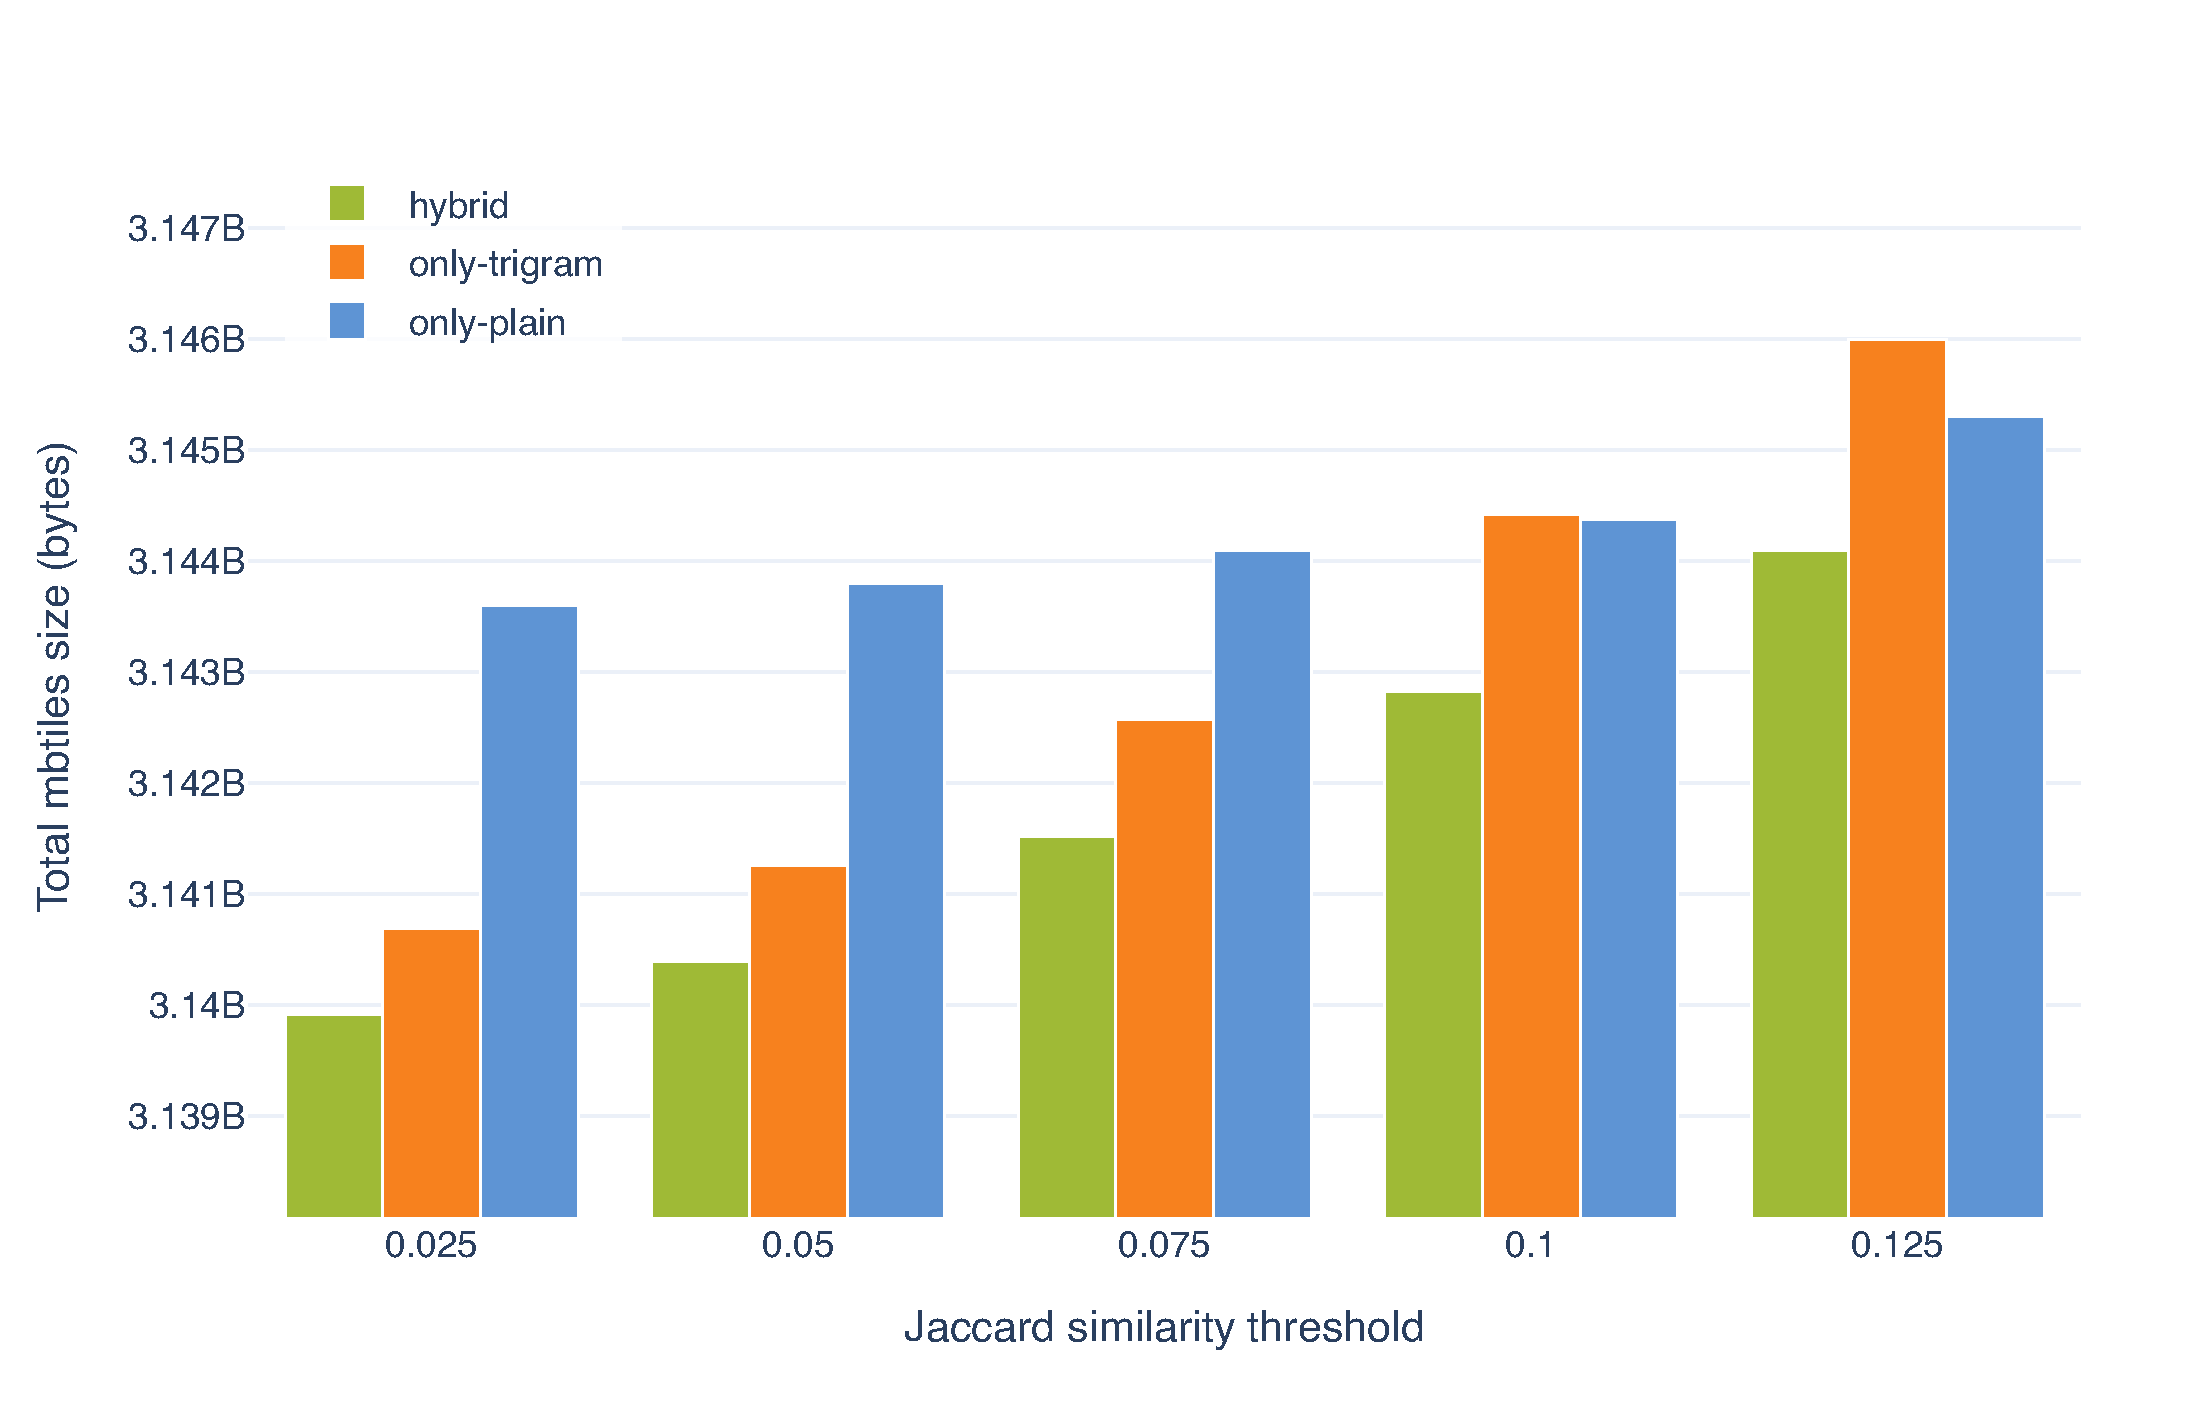
\includegraphics[width=\linewidth]{figures/minhash_sweep.pdf}
    \caption{Total encoded mbtiles size of the Germany OpenMapTiles tileset under different MinHash similarity modes and Jaccard thresholds.  Lower is better.  The hybrid mode (teal) produces the smallest output at every threshold; all modes increase monotonically with threshold as fewer column pairs qualify for shared-dictionary grouping.  The y-axis is zoomed to the data range to make the differences visible; the full range spans approximately \qty{6}{\mega\byte} out of \qty{3.14}{\giga\byte} total}
    \label{fig:minhash_sweep}
\end{figure}

\paragraph{Geometry and ID encoding}
Geometry vertices are encoded as either \emph{componentwise deltas} (CWD) or \emph{Morton-code dictionaries}.
CWD encodes each vertex as the delta from the previous vertex, producing a single interleaved stream $[x_0, y_0, \Delta x_1, \Delta y_1, \ldots]$ that is then compressed via the per-stream integer competition.
The Morton-code dictionary approach computes a Z-order code for each unique vertex pair, stores the deduplicated codes as a sorted dictionary, and references them via per-vertex offset indices - producing two streams (offsets and dictionary deltas) instead of one.
The encoder tries both strategies (when the coordinate range permits Morton encoding, i.e., both axes fit within 16~bits after shifting) and retains the smaller result.
Feature IDs are encoded through the same per-stream integer competition as other integer columns, using an explicit \texttt{IdWidth} tag (\texttt{Id32} or \texttt{Id64}) to select the physical word width.
The \ac{FastPFOR} codec operates on 32-bit blocks by construction, so only 32-bit ID streams and property columns reach it; 64-bit streams fall back to \ac{VarInt} (the \ac{VarInt} candidate list covers both widths).
The encoder chooses \texttt{Id32} when the maximum observed ID fits in \texttt{u32}, narrowing 64-bit-declared ID columns whose actual values fit in 32 bits; the round-trip correctness of this narrowing is covered by per-case tests including \texttt{test\_config\_produces\_correct\_variant} and proptest round-trips over $[0,\,\texttt{u32::MAX}]$ and $[0,\,\texttt{u64::MAX}]$ domains.
Structural patterns (sequential, constant) are discovered by the same data profiler that drives the inner competition: sequential IDs reach DeltaRle, constant IDs reach \ac{RLE}, and short or irregular sequences fall back to plain \ac{VarInt}.

\paragraph{Encoder cost amortisation}
Multi-trial encoding is made affordable through warm-start caching - \ac{FSST} compressors, Morton metadata, and vertex-strategy decisions are computed once and reused across sort trials.
Furtermore, scratch buffers grow on first use and are recycled.

The alternatives mechanism is an RAII stack of \texttt{AltSession} guards: each candidate writes into a sub-range of the encoder's buffers, and the guard's \texttt{Drop} impl retains only the bytes of the smallest candidate and rolls the cursor back for the others, so nesting lets the inner per-stream competition resolve before the enclosing sort-strategy trial commits.

\paragraph{Encoder correctness validation}
\begin{sloppypar}
    Because \ac{FastPFOR} explicitly disclaims input validation and the encoder performs narrowing, run-encoding, and dictionary rebuilds that each have independent failure modes, the encoder is validated by a multi-layer test harness:
    (i)~an in-tree proptest suite covering every \texttt{IntEncoder} variant, with round-trip assertions across the full representable range of the selected physical type;
    (ii)~a libFuzzer harness that fuzzes full \texttt{DecodedLayer} round-trips, with a corpus accumulated over previous runs;
    (iii)~snapshot tests via \texttt{insta} for the per-stream profiler's candidate lists, pinning the pruning heuristics to known-good outputs; and
    (iv)~the pixel-exact visual validation described in \cref{sec_visual_correctness}, which exercises the full decode path against a known-good baseline.
\end{sloppypar}

\subsection{Metadata Optimisations}\label{sub_metadata_optimisations}

Metadata optimisations provide the client with more accurate information, enabling it to skip unnecessary work during rendering.
\cref{tab:metadata_passes} summarises the implemented techniques.

\begin{table}[htbp]
    \centering
    \begin{tblr}{
            colspec = {p{3.8cm} p{1.8cm} p{9.5cm}},
            rows = {font=\small},
            row{1} = {font=\small\bfseries},
        }
        \toprule
        Pass & Data & Description \\
        \midrule
        Dead source elimination & none      & Remove sources that are no longer referenced after dead layer elimination \\
        Metadata refinement     & sampling  & Provide accurate \texttt{minzoom}/\texttt{maxzoom} bounds derived from filter analysis and tile statistics \\
        \bottomrule
    \end{tblr}
    \caption{Metadata-level optimisations techniques.}
    \label{tab:metadata_passes}
\end{table}

\subsection{Tile Statistics Collection}\label{sub_tile_statistics}

Several optimisations passes - stats-driven constant folding, dead elimination with geometry-type mismatch, metadata refinement, selectivity reordering, and the tile pruning advisory - require knowledge of the actual tile data.
This knowledge is provided by a statistics collection phase that scans the tile set and produces a per-source, per-source-layer statistical profile.

For each source layer, the following statistics are collected:

\begin{itemize}
    \item \textbf{Feature count}: total number of features across all tiles (note: features appearing in multiple tiles at different zoom levels are counted multiply, as the optimiser reasons per-tile, not per-geographic-entity).
    \item \textbf{Features by zoom}: a per-zoom-level feature count, used by metadata refinement to determine the first and last zoom level at which data exists.
    \item \textbf{Geometry types}: counts of Point, LineString, and Polygon features, used by dead elimination to detect geometry-type mismatches.
    \item \textbf{Feature ID presence}: whether any feature carries a non-zero feature ID, used by the advisory to decide whether to strip the ID column.
    \item \textbf{Per-property statistics}: for each property name, the statistics depend on the wire type:
    \begin{itemize}
        \item \emph{Boolean}: present count and true count.
        \item \emph{Integer/unsigned integer}: present count, minimum, maximum, cardinality, and (if cardinality $\leq 200$) a full value-frequency map.
        \item \emph{Double}: present count, minimum, maximum, cardinality (no value-frequency map, since floating-point equality is unreliable for folding).
        \item \emph{String}: present count, cardinality, and (if cardinality $\leq 200$) a value-frequency map sorted by descending frequency.
    \end{itemize}
\end{itemize}

Statistics can be collected at a configurable \emph{sample rate}.
A sample rate of~1.0 (full census) is required for irreversible decisions such as dead layer elimination or property interning; lower sample rates are sufficient for selectivity estimation and reordering.
This distinction is enforced by a sample-rate guard in the optimiser: passes that permanently remove data check that the sample rate is~1.0 before applying.

\section{Gathering a Representative Sample}\label{sec_gathering_sample}

Evaluating an optimiser requires both a diverse set of styles and realistic tile data.
We employ a two-tier strategy.

\subsection{Benchmarking Corpus}\label{sub_deep_corpus}

For rendering benchmarks that require tile data and animated camera scenarios, we curated a corpus of 15 publicly available styles that use the OpenMapTiles or BasemapDE schema:

\begin{itemize}
    \item \textbf{4 OpenFreeMap styles}: liberty, bright, positron, fiord.
    \item \textbf{7 OpenMapTiles community styles}: dark-matter, osm-bright, klokan-basic, toner, osm-liberty, americana, stadia-outdoors.
    \item \textbf{4 Government and institutional styles}: ICGC~fosc, ICGC~gris, Basemap\-DE topo\-graphic, Basemap\-DE colour.
\end{itemize}

These styles span a range of complexity-from minimal basemaps with fewer than 50~layers to verbose institutional styles with several hundred layers-and exercise different subsets of the expression language.

\subsection{Generalisation Corpus}\label{sub_generalisation_corpus}

To assess whether optimisations gains generalise beyond the deep corpus, we collected 13 styles from the Maputnik style editor catalogue (two additional catalogue entries were unavailable at the time of measurement).
These styles are evaluated using static analysis only (style size, complexity metrics, pass applicability) and do not require tile data.

\subsection{Tile Data and Caching}\label{sub_tile_data}

Tile data is sourced from \ac{OSM} via Planetiler or the German government.
Both sources are consumed through the standard Web Mercator XYZ tiling scheme used by MapLibre, so all zoom-level reasoning in the thesis assumes this grid; BasemapDE is accessed through its XYZ-compatible endpoint rather than its native \acs{WMTS} grid, ensuring that the optimiser's tile indexing is uniform across the corpus.
Only for \ac{OSM} is the underlying data fully available, so only for this source can tile statistics be collected at a sample rate of~1.0.
To ensure reproducibility across benchmark runs, all tile requests are routed through a local caching proxy that stores tiles on first access and replays them on subsequent runs with the latency and download speed of a 4G internet connection according to Rusan et al.~\cite{rusanAssessmentPacketLatency2015} ($\text{size} / 30\frac{Mb}{s} + 25ms$).
This eliminates network variability and guarantees that every ablation step operates on identical tile data (after an initial, discarded run).

All compressed-size measurements throughout this thesis use maximum compression: gzip level~9, Brotli quality~11, and zstd level~22.
This reflects the deployment scenario where tiles and styles are compressed once and served many times, so encoding cost is negligible relative to the number of requests served.

\subsection{Geographic and Use-Case Scenarios}\label{sub_scenarios}

The benchmark harness defines 18 scenarios drawn from a matrix of 15 geographic locations and 5 camera animation types:

\begin{itemize}
    \item \textbf{Locations} span high-density cities with Latin scripts (Munich, Berlin, Paris, New York, Rome), cities with non-Latin scripts (Tokyo, Beijing, Seoul, Cairo), and low-density or special nature regions (Black Forest, Amazon, Swiss Alps, Sahara, Venice, Stockholm Archipelago).
    \item \textbf{Animations} exercise different rendering workloads:
    \emph{zigzag} alternates zoom levels while panning;
    \emph{spiral} traces a circle at constant zoom with rotating bearing;
    \emph{zoomdrill} zooms from overview to street level and back;
    \emph{pansweep} sweeps across a region at constant zoom;
    \emph{bearingspin} rotates bearing at high pitch.
\end{itemize}

Each scenario is a specific (location, animation) pair.
The full cross-product of 15 locations and 5 animations is 75 pairs, which is too expensive to run for every ablation step (each cell requires 15 repeat runs for statistical validity across 17 ablation steps and 15 styles, giving roughly $75 \times 15 \times 17 \times 15 = \num{286875}$ full animations).
The 18 selected scenarios are chosen by stratified sampling so that every location appears at least once and every animation appears at least three times, and so that all combinations of density class (high/low) and script class (Latin/non-Latin) are represented.
Within each stratum the specific (location, animation) pair is the one that exercises the most layers in the densest style in the corpus, ensuring that the sample is biased \emph{against} the null hypothesis of \enquote{no effect} - i.e.\ towards scenarios where any rendering-cost differences are most likely to be visible.
This is a convenience sample by design:
it is not claimed to be unbiased across all real-world usage patterns, but it is claimed to be a reasonable stress test of the optimiser across the dimensions (density, script, zoom trajectory, camera motion) that most plausibly interact with style and data-level optimisations.

\section{Evaluation}\label{sec_evaluation}

Since many of the investigated optimisations techniques have not previously been studied in the context of map rendering pipelines, their effectiveness must be evaluated empirically.
The evaluation considers several dimensions:

\begin{itemize}
    \item \textbf{Data savings}: reduction in style size (raw, gzip, and Brotli) and tile transfer volume.
    \item \textbf{Rendering performance}: client-side metrics including load time, frames per second, frame time percentiles (p50, p95, p99), jank count, style parse time, time to first tile, and time to first frame.
    \item \textbf{Optimisation cost}: preprocessing time introduced by each pass, measured as wall-clock time on the optimiser's host machine; this is an offline cost amortised over all subsequent tile deliveries.
    \item \textbf{Efficiency}: \emph{qualitative} discussion of the energy implications of reduced data transfer and fewer rendering operations.  No direct power or energy measurement (RAPL, battery delta) is performed, because the benchmark harness runs on a desktop workstation rather than a battery-constrained mobile device; any quantitative energy claim would require a different hardware platform and is deferred to future work.
\end{itemize}

\subsection{Metrics}\label{sub_metrics}

The benchmark harness collects the following metrics per run:

\begin{itemize}
    \item \textbf{Load time} (\texttt{loadMs}): wall-clock time from requesting the map to completion of the initial render, including style parsing, tile fetching, tile decoding, and first paint.
    Within the rendering benchmark, decoding latency is embedded in \texttt{loadMs} rather than isolated, because the browser-based harness cannot separate decoder wall-clock time from the surrounding fetch and first-paint work without renderer-internal instrumentation.
    Isolated decoding throughput is instead measured via Criterion micro-benchmarks on the Rust decoder (\cref{tab:decode_throughput}).
    \item \textbf{Style parse time} (\texttt{styleParseMs}): time spent parsing and compiling the style JSON into the renderer's internal representation.
    \item \textbf{Time to first tile} (\texttt{firstTileMs}): time from map initialisation until the first tile is decoded and ready for rendering.
    \item \textbf{Time to first frame} (\texttt{firstFrameMs}): time until the first frame is composited and presented.
    \item \textbf{Frames per second} (\texttt{fps}): average rendering throughput during the animation phase.
    \item \textbf{Frame time percentiles} (\texttt{p50}, \texttt{p95}, \texttt{p99FrameMs}): distribution of per-frame render times, capturing both typical and worst-case latency.
    \item \textbf{Jank count} (\texttt{jankCount}): number of frames exceeding \qty{16.67}{\milli\second} (the 60\,\ac{FPS} budget), indicating visible stuttering.
    \item \textbf{Heap memory} (\texttt{heapUsedMB}, \texttt{peakHeapMB}): JavaScript heap usage during the benchmark, capturing the memory cost of style structures and tile data.
    \item \textbf{Idle time} (\texttt{idleMs}): time the renderer spends idle (waiting for tiles or GPU sync), indicating headroom.
\end{itemize}

\noindent Additionally, the following static metrics are computed for each optimised style without running the renderer:

\begin{itemize}
    \item \textbf{Style size}: raw byte count, gzip-compressed size, and Brotli-compressed size.
    \item \textbf{Complexity metrics}: total \ac{AST} node count, maximum expression depth, layer count, filter count, and expression operator histogram.
\end{itemize}

\subsection{Ablation Methodology}\label{sub_ablation}

The primary evaluation methodology is cumulative ablation: passes are added one at a time in a fixed order, and the full benchmark suite is re-run after each addition.
This reveals both the marginal contribution of each pass and the interactions between passes.
The ablation comprises 17~steps: a baseline (no optimisations) followed by 16~passes added incrementally in the order listed in \crefrange{tab:expression_passes}{tab:data_passes}.

Each scenario/style combination is executed for 15~runs.
The median and standard deviation of each metric are reported; the median is preferred over the mean because rendering performance distributions are right-skewed (occasional long frames inflate the mean).
To reduce measurement noise, the benchmark harness pins rendering to real GPU hardware via ANGLE/Vulkan rather than the software rasteriser used for pixel-exact render tests.
This ensures that GPU-bound workloads (fragment shading, texture sampling, blend operations) are measured realistically.

All tile requests are served from a local caching proxy that stores tiles on first access and replays them on subsequent runs.
To avoid artificially high performance from local network transfer, the proxy introduces a network delay that simulates realistic latency.
Concretely, each tile response is delayed by a fixed per-request round-trip time on top of a per-byte throughput throttle, so the wire time for a tile of $b$ bytes is approximately $\mathrm{RTT} + b / \mathrm{bandwidth}$.
Both values are configurable; the default benchmark run uses an \ac{RTT} of \qty{25}{\milli\second} and a bandwidth cap of \qty{30}{\Mbps}, matching the 4G profile of Rusan et al.~\cite{rusanAssessmentPacketLatency2015}.
The model does not simulate packet loss, HTTP/2 multiplexing, TCP slow-start, or HTTP/3 (QUIC) with its 0-RTT connection resumption and absence of head-of-line blocking - all of which would amplify the benefit of smaller tiles - so the measured load-time improvements from tile shaving are a conservative lower bound on what a real deployment would observe.
This ensures that tile-fetch improvements (e.g.\ smaller tiles due to shaving) are measured under conditions representative of a \ac{CDN}-served deployment while remaining deterministic across runs.

The benchmark harness itself is a Puppeteer-driven headless browser that programmatically loads the MapLibre GL~JS renderer, applies a camera animation scenario, and collects performance counters via the \texttt{Performance} API and custom instrumentation hooks in the renderer.

Visual correctness is verified separately through pixel-exact render tests that compare optimised output against the unoptimised baseline across a grid of zoom levels and geographic locations.
These tests use a software rasteriser to ensure deterministic pixel output, independent of GPU driver differences.

With the optimiser pipeline, its individual passes, and the evaluation methodology now defined, the following chapter applies this methodology to evaluate each optimisation category - expression-level, structural, and data-level - and then analyses their combined effect across the full benchmark corpus.
